\section{Experiments}
Write some intro text here
\subsection{Setup}
We conduct experiments the the StyleGAN2-ADA \cite{karras2020training} generator (config-F), trained on the FFHQ \cite{karras2019style} (resolution 1024) dataset.


\subsection{Optimal Generator Architecture}




In \cref{fig:comparison} we compare our method to~\cite{yao2021latent}, the current state-of-the-art in semantic editing of faces in videos. 
%When working on their simpler scenes, our method maintains improved identity and avoids pitfalls like the appearance of artifacts around stitching regions. 
When evaluating their method on our more challenging scenes, we observe considerable quality degradation and loss of temporal coherence. Our method, in contrast, maintains high fidelity and consistent editing without relying on any explicit temporal smoothing.
Note in particular the blurry artifacts induced by \cite{yao2021latent} when blending the shirt. Moreover, the employment of optimization-based PTI results in the age changing between the different frames.

% Due to the inconsistency between the pivots, different frames are affected differently by the editing which leads to an unrealistic outcome.

% \begin{figure*}
%     \centering
%     \setlength{\belowcaptionskip}{-6pt}
%     \setlength{\tabcolsep}{0.5pt}
%     {
%     \begin{tabular}{ccccccccccc}
        
%         \vspace{-0.0615cm}
        
%         % % Identity 1

%         % \raisebox{0.12in}{\rotatebox{90}{Original}} &
%         % 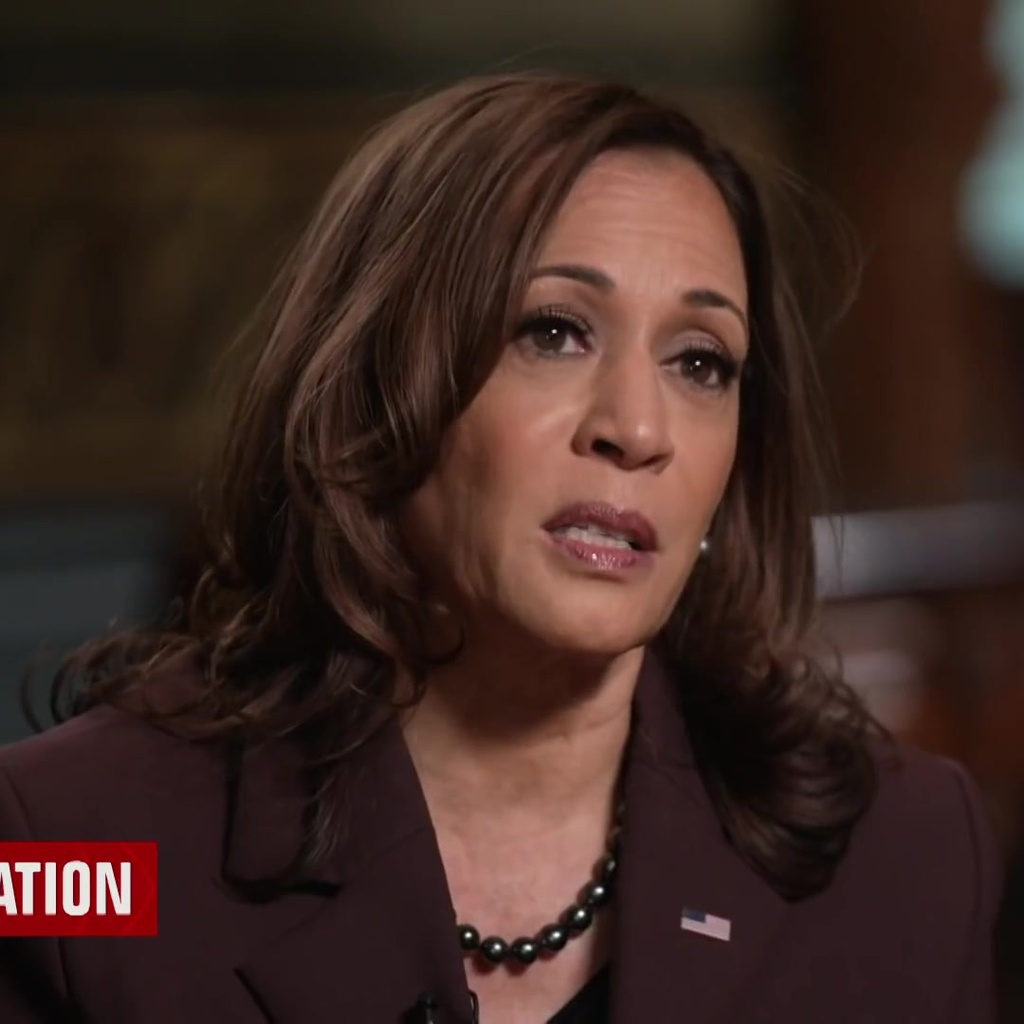
\includegraphics[width=0.095\textwidth]{resources/images/harris/original/source_0027.jpeg} &
%         % 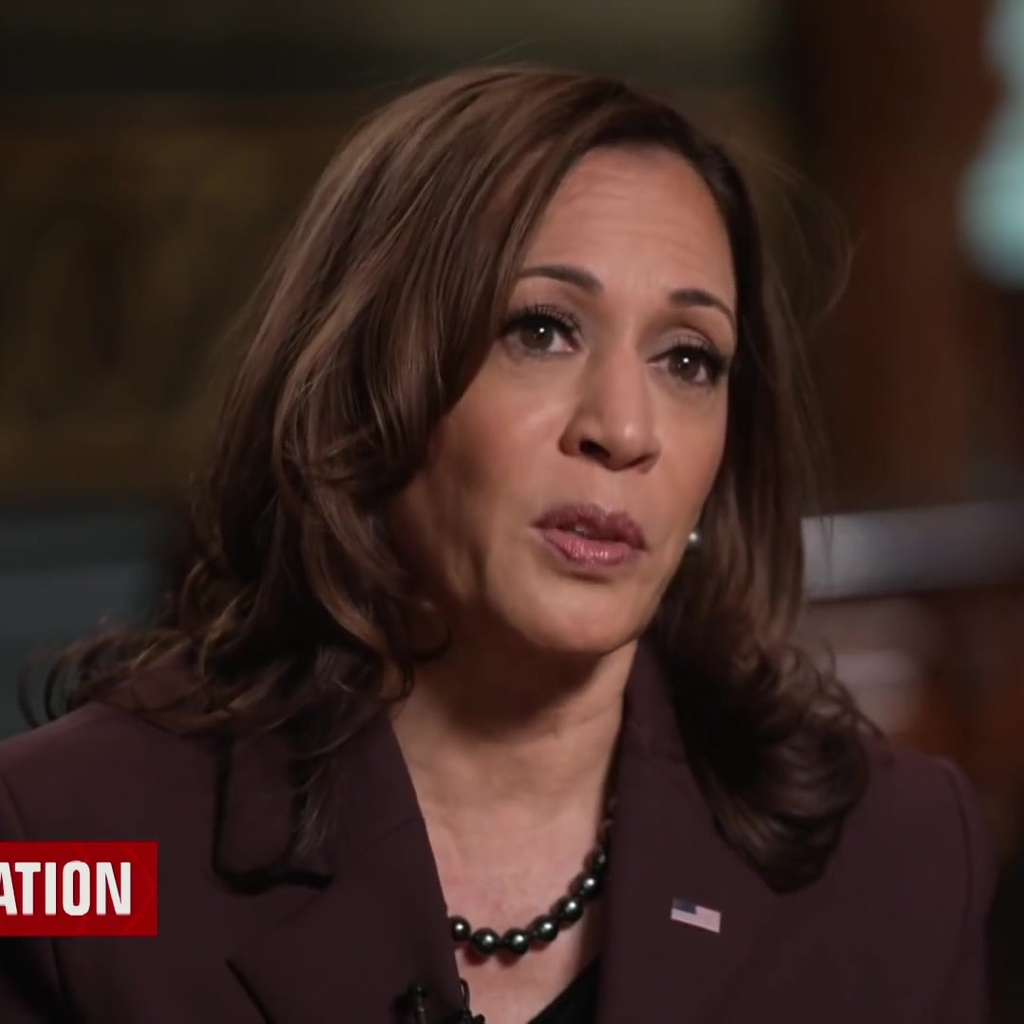
\includegraphics[width=0.095\textwidth]{resources/images/harris/original/source_0046.jpeg} &
%         % 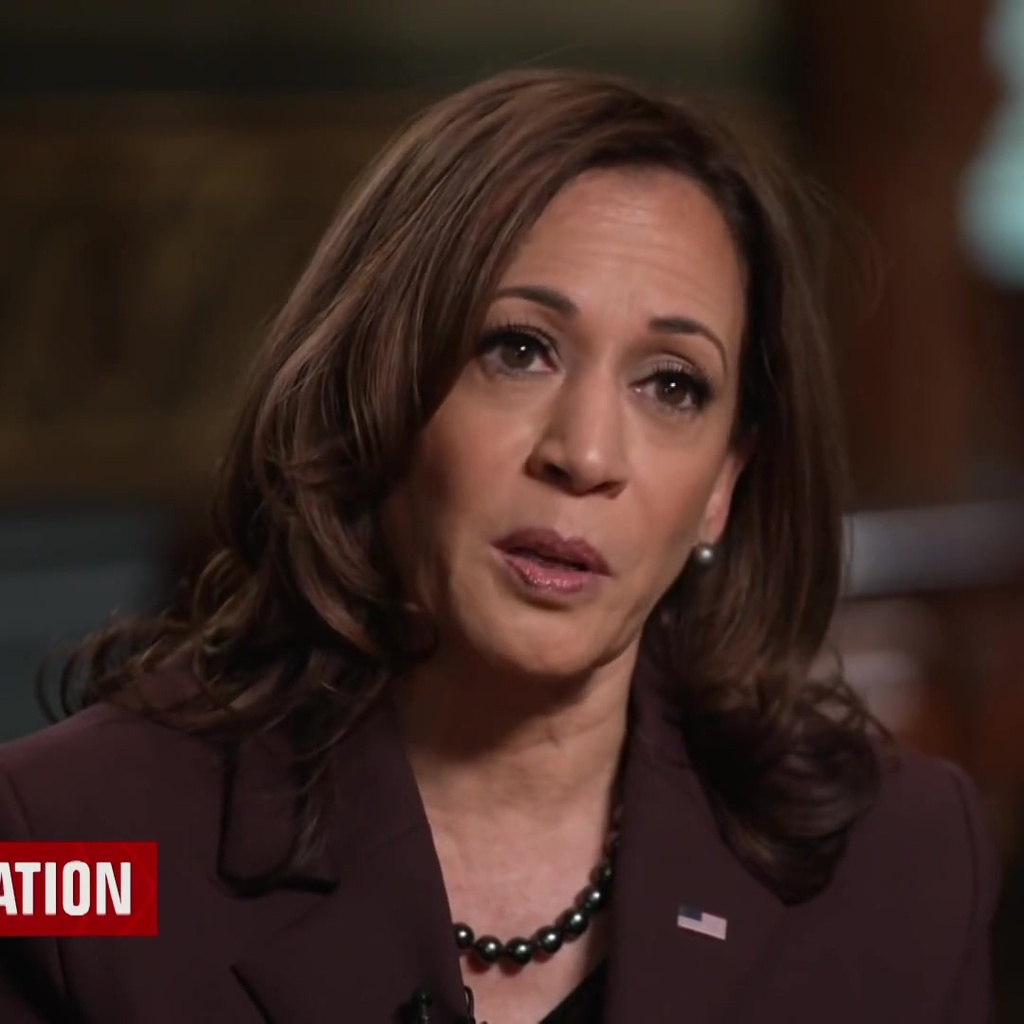
\includegraphics[width=0.095\textwidth]{resources/images/harris/original/source_0058.jpeg} &
%         % 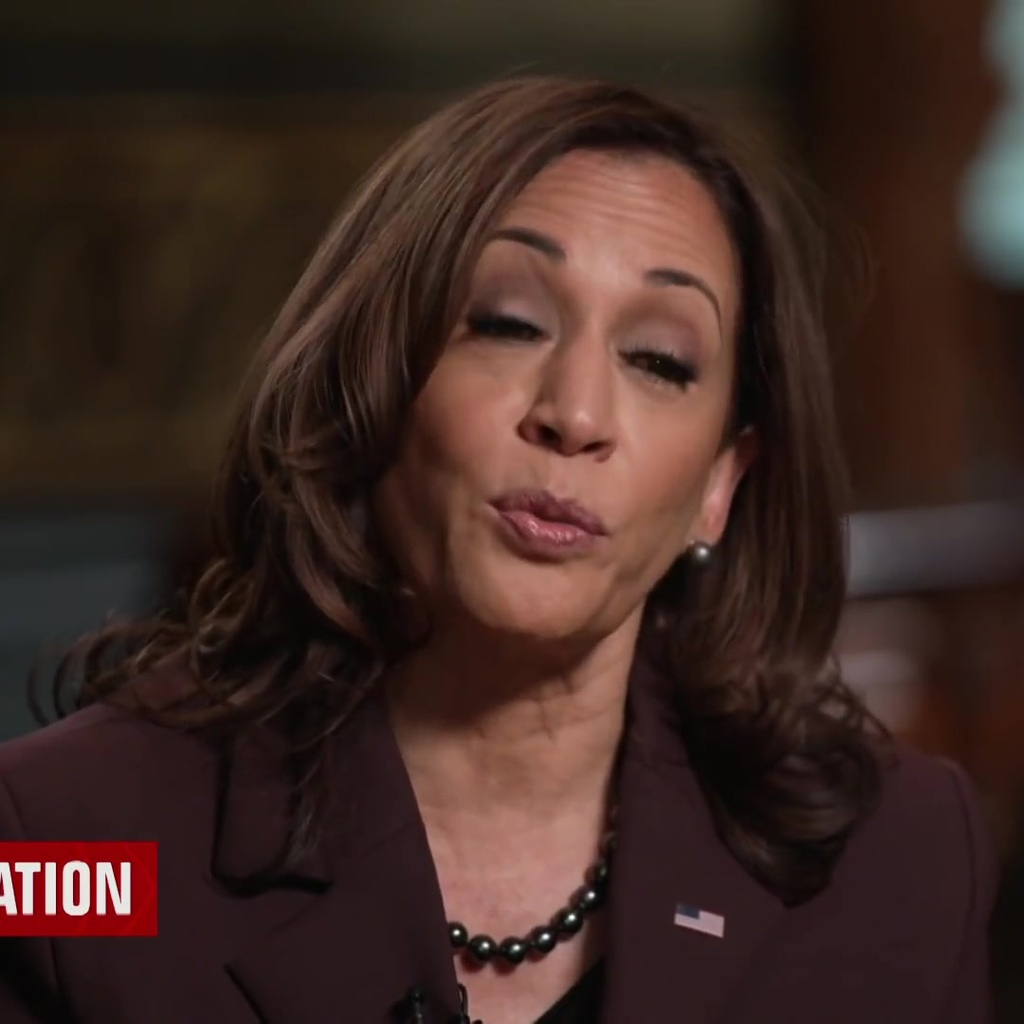
\includegraphics[width=0.095\textwidth]{resources/images/harris/original/source_0077.jpeg} &
%         % 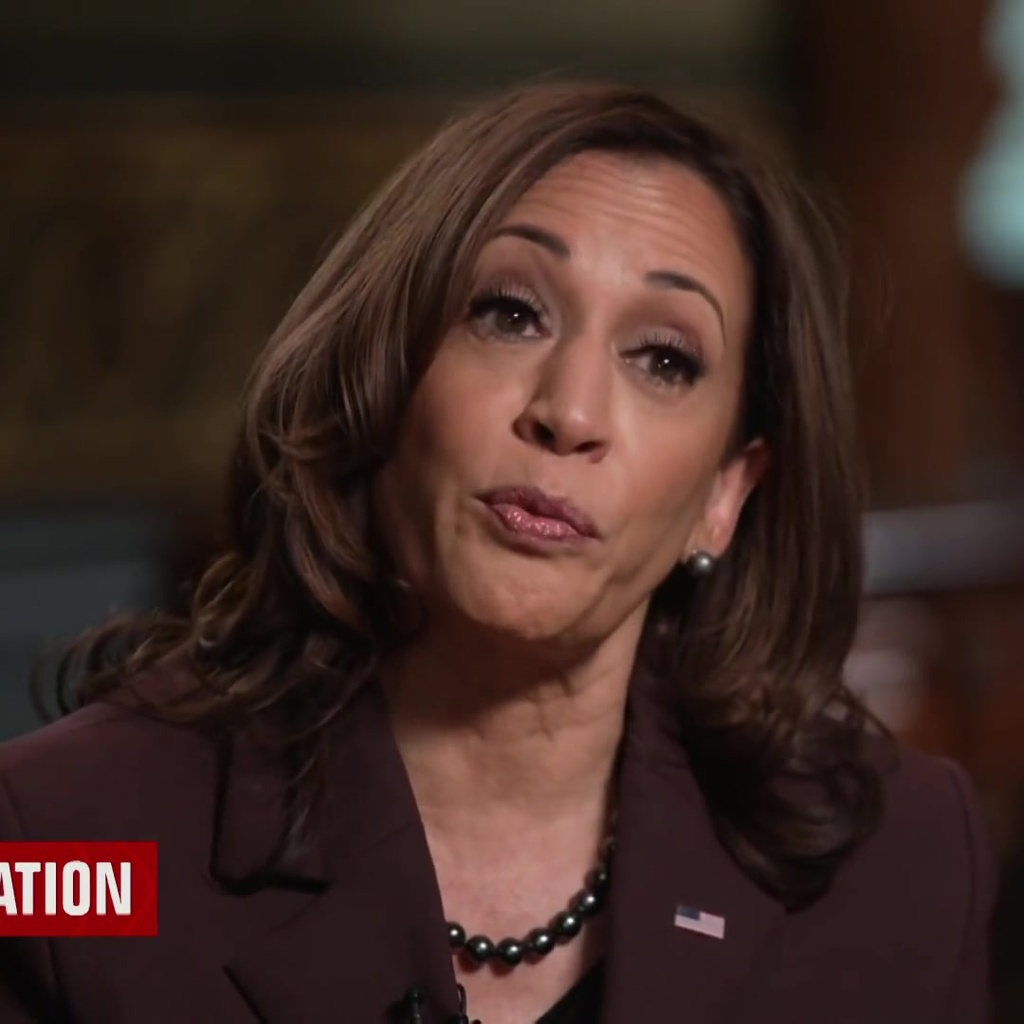
\includegraphics[width=0.095\textwidth]{resources/images/harris/original/source_0082.jpeg} &
%         % 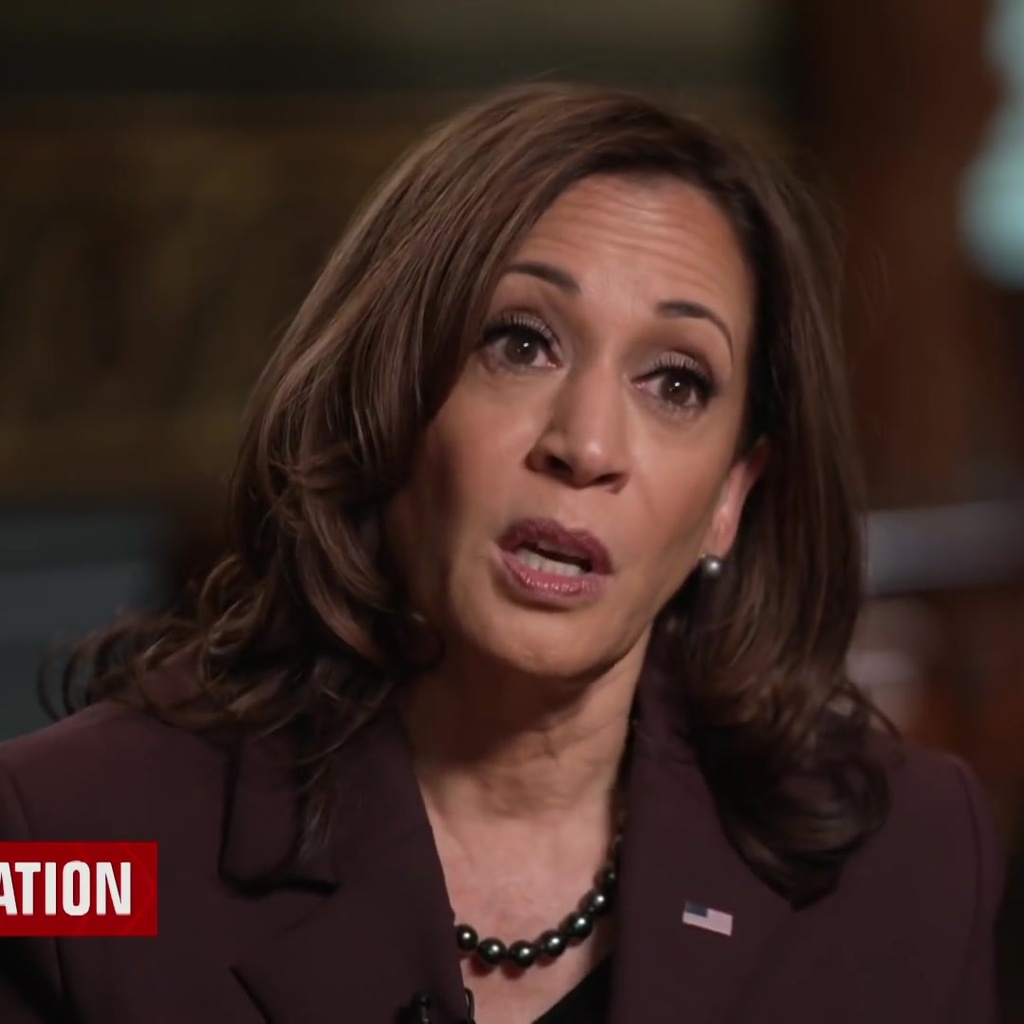
\includegraphics[width=0.095\textwidth]{resources/images/harris/original/source_0103.jpeg} &
%         % 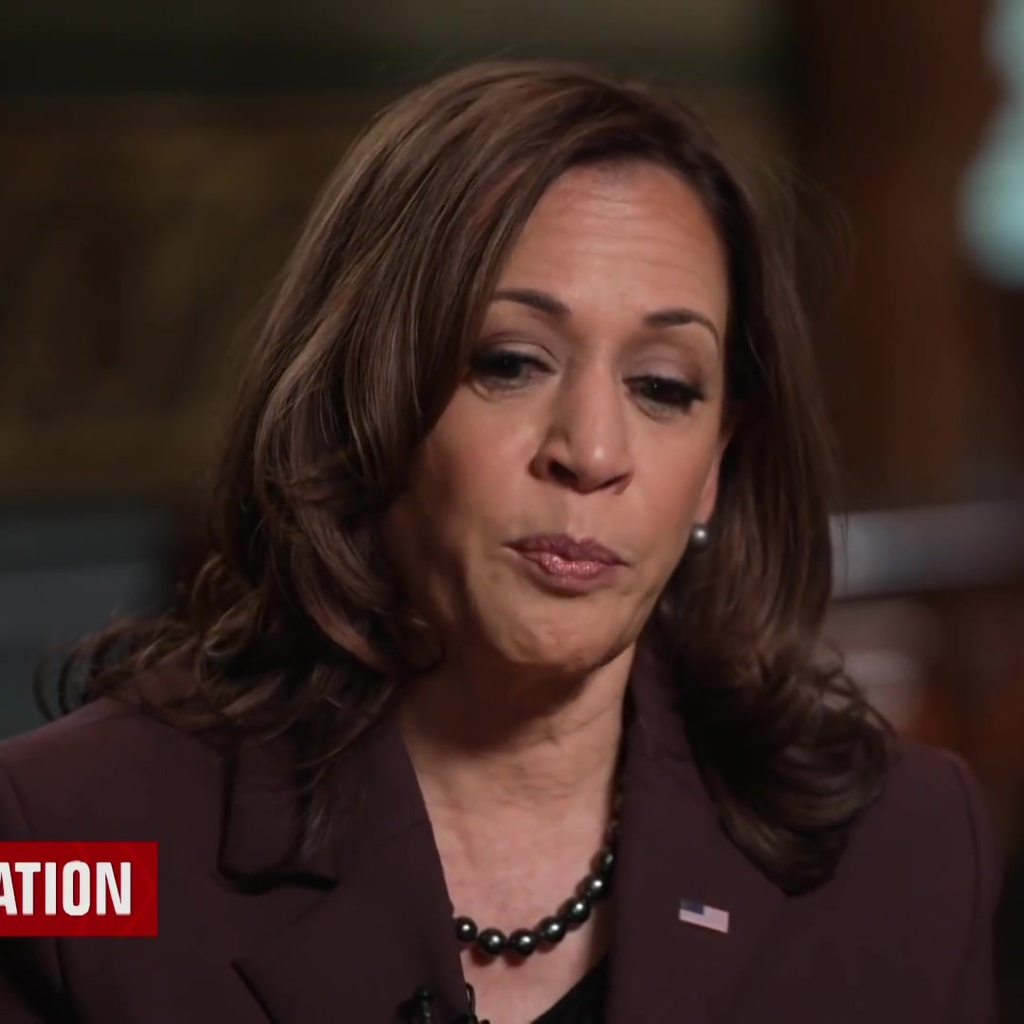
\includegraphics[width=0.095\textwidth]{resources/images/harris/original/source_0122.jpeg} &
%         % 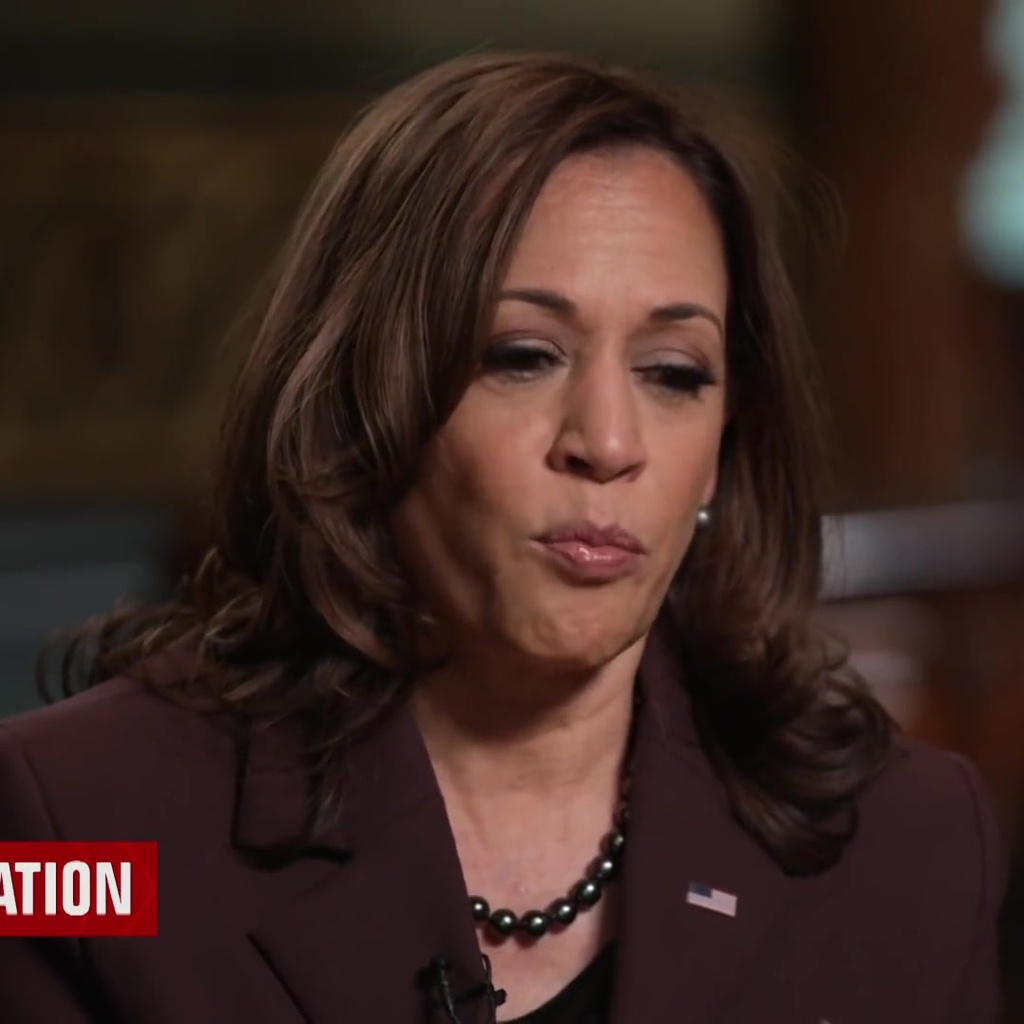
\includegraphics[width=0.095\textwidth]{resources/images/harris/original/source_0164.jpeg} &
%         % 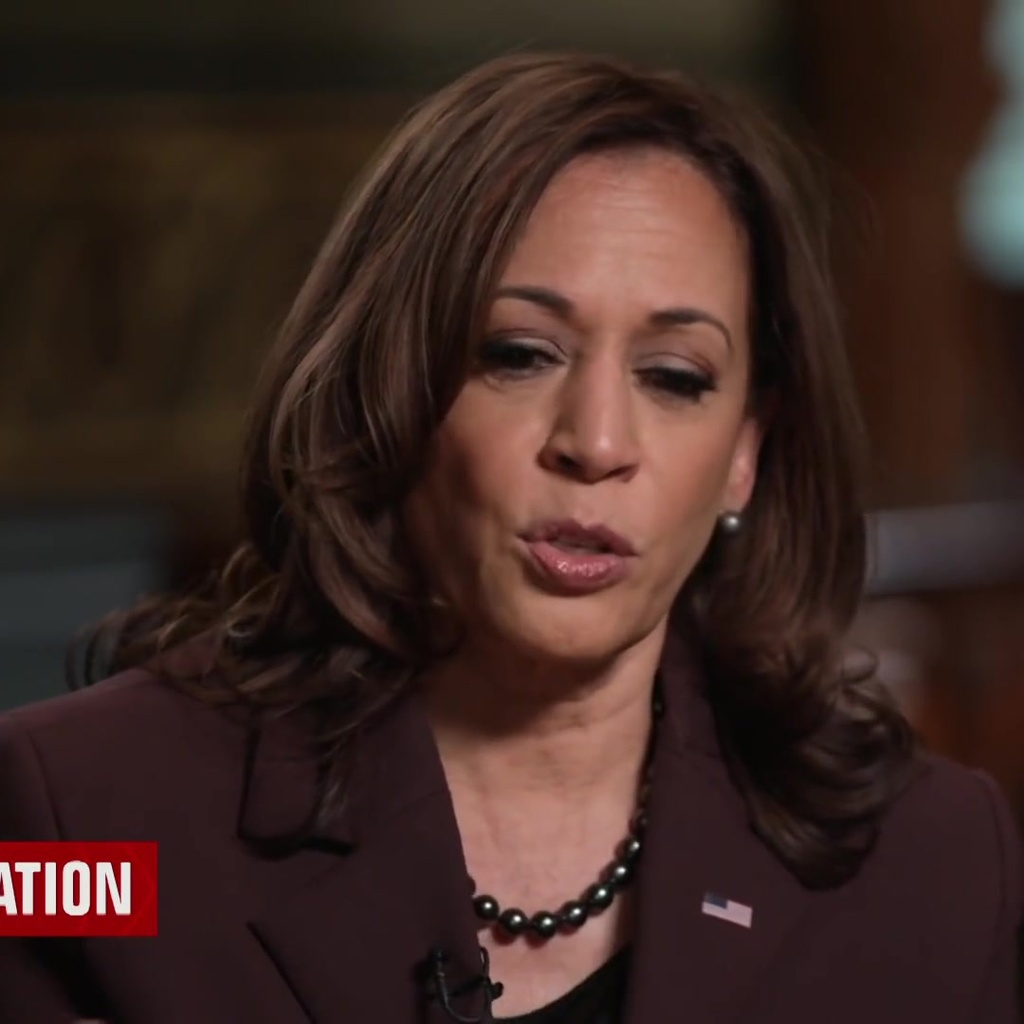
\includegraphics[width=0.095\textwidth]{resources/images/harris/original/source_0178.jpeg} &
%         % 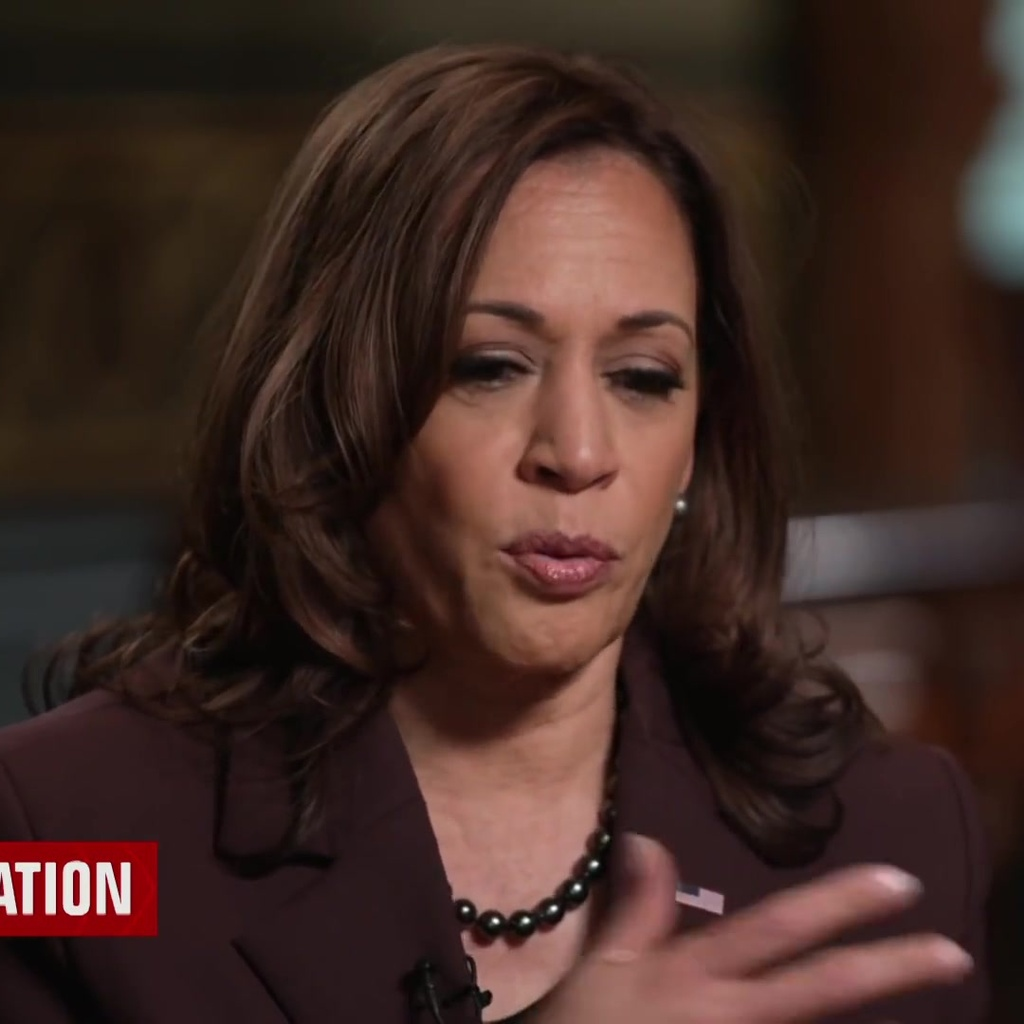
\includegraphics[width=0.095\textwidth]{resources/images/harris/original/source_0195.jpeg} \\
        
%         % \raisebox{0.18in}{\rotatebox{90}{$+Smile$}} &
%         % 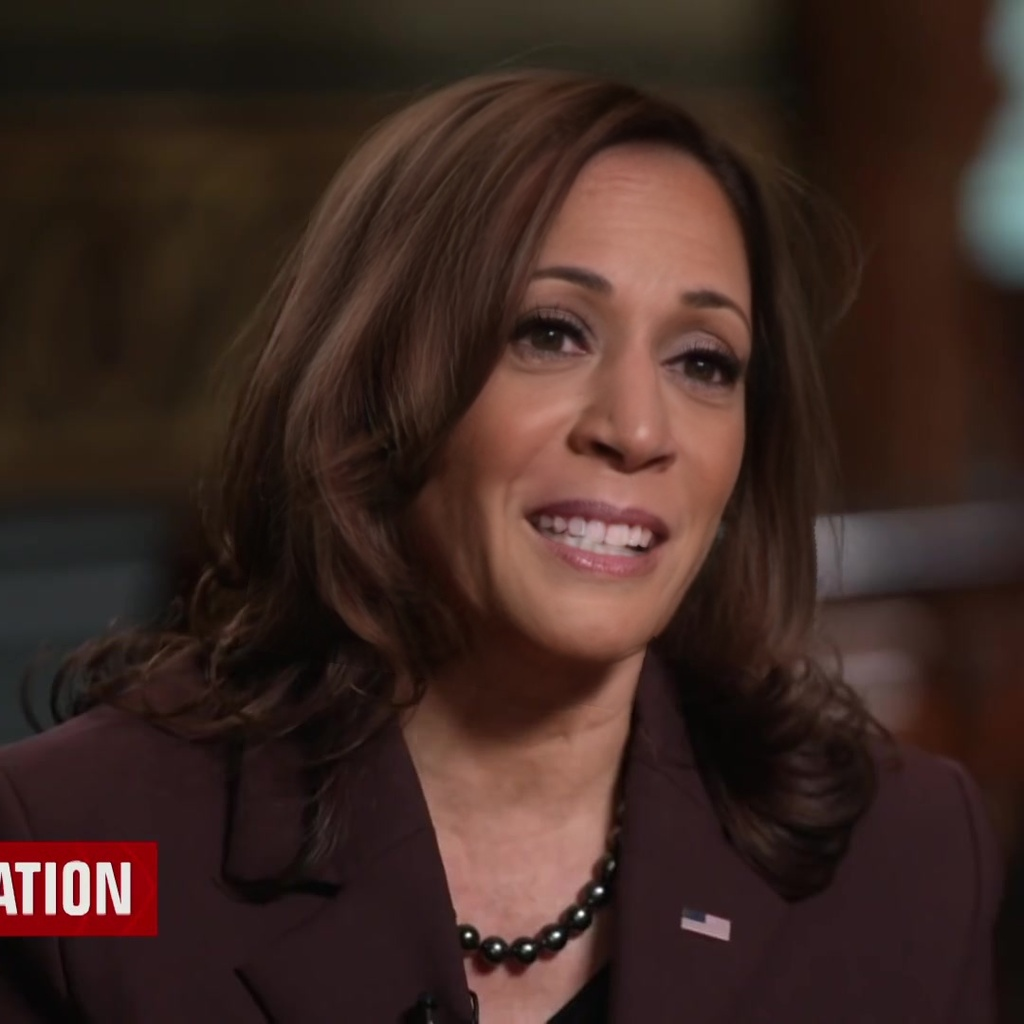
\includegraphics[width=0.095\textwidth]{resources/images/harris/smile/edit_0027.jpeg} &
%         % 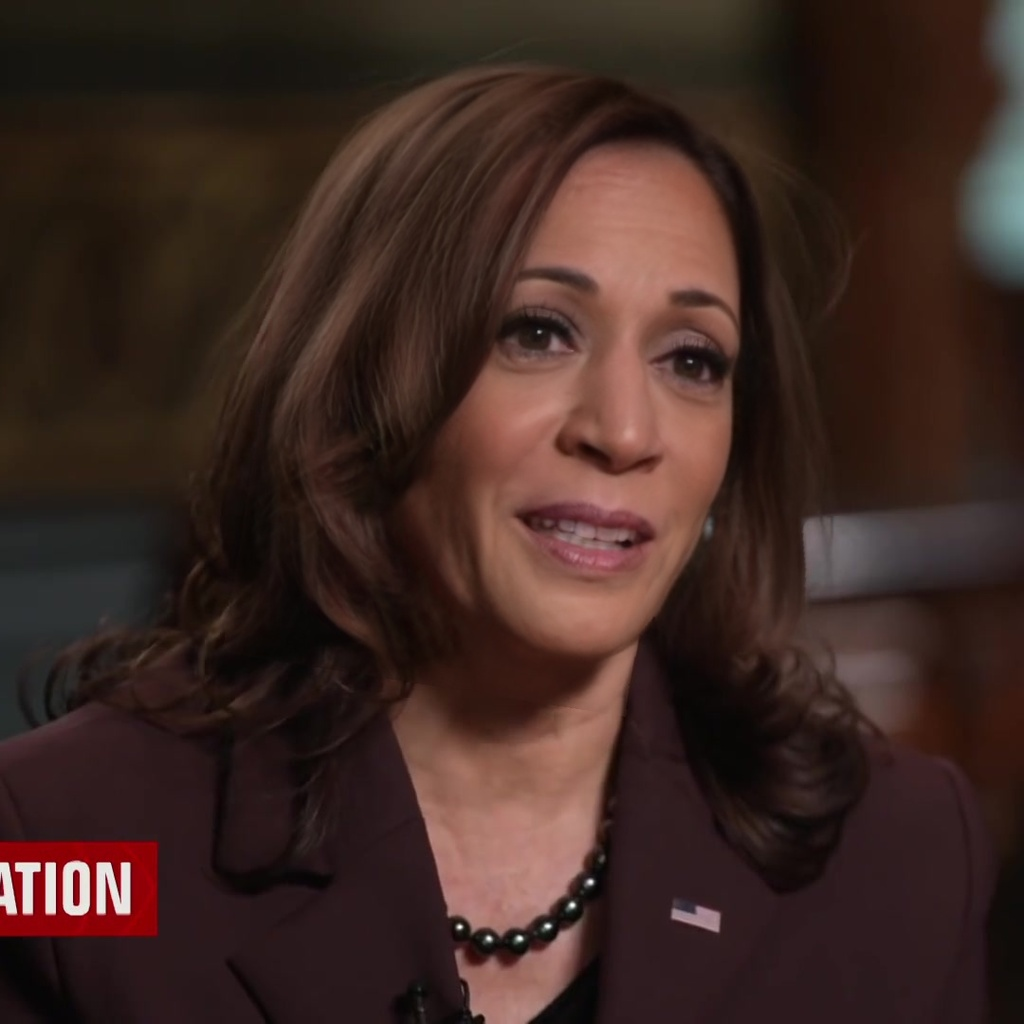
\includegraphics[width=0.095\textwidth]{resources/images/harris/smile/edit_0046.jpeg} &
%         % 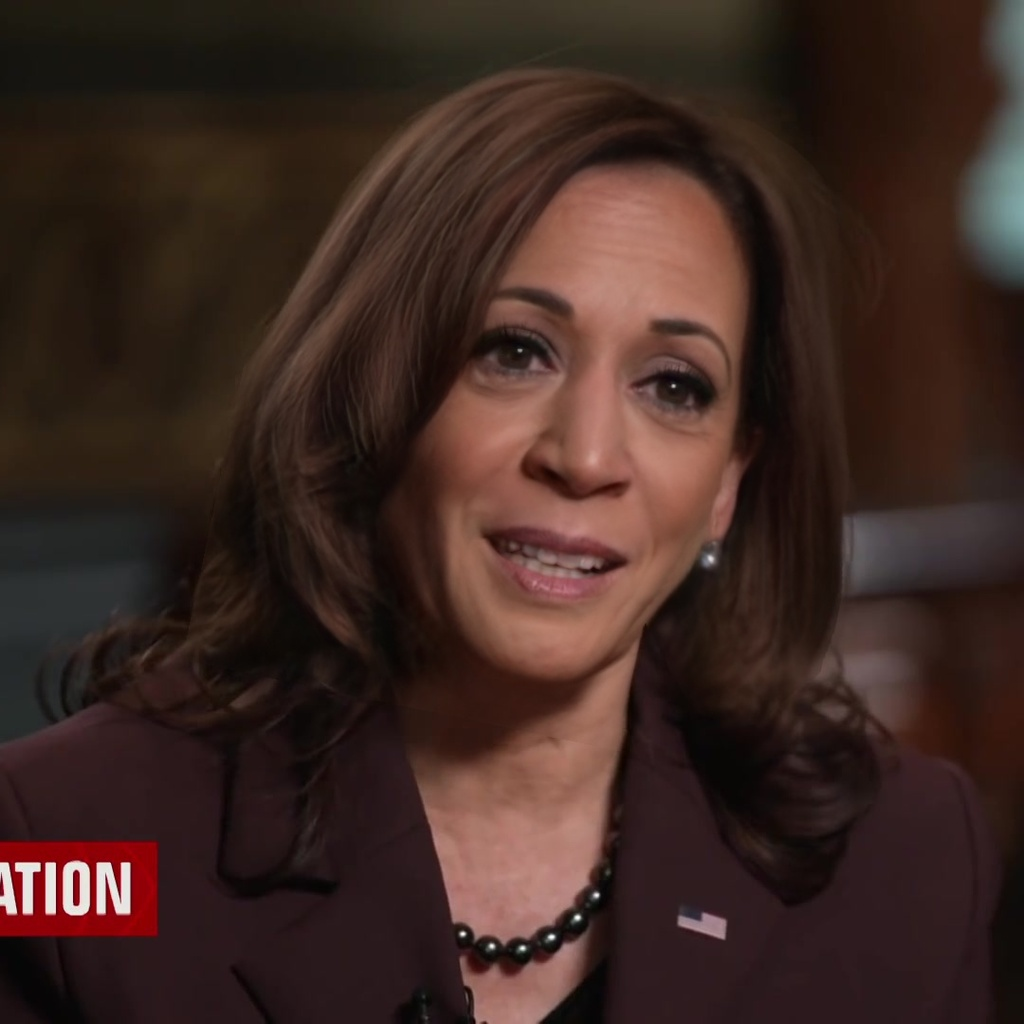
\includegraphics[width=0.095\textwidth]{resources/images/harris/smile/edit_0058.jpeg} &
%         % 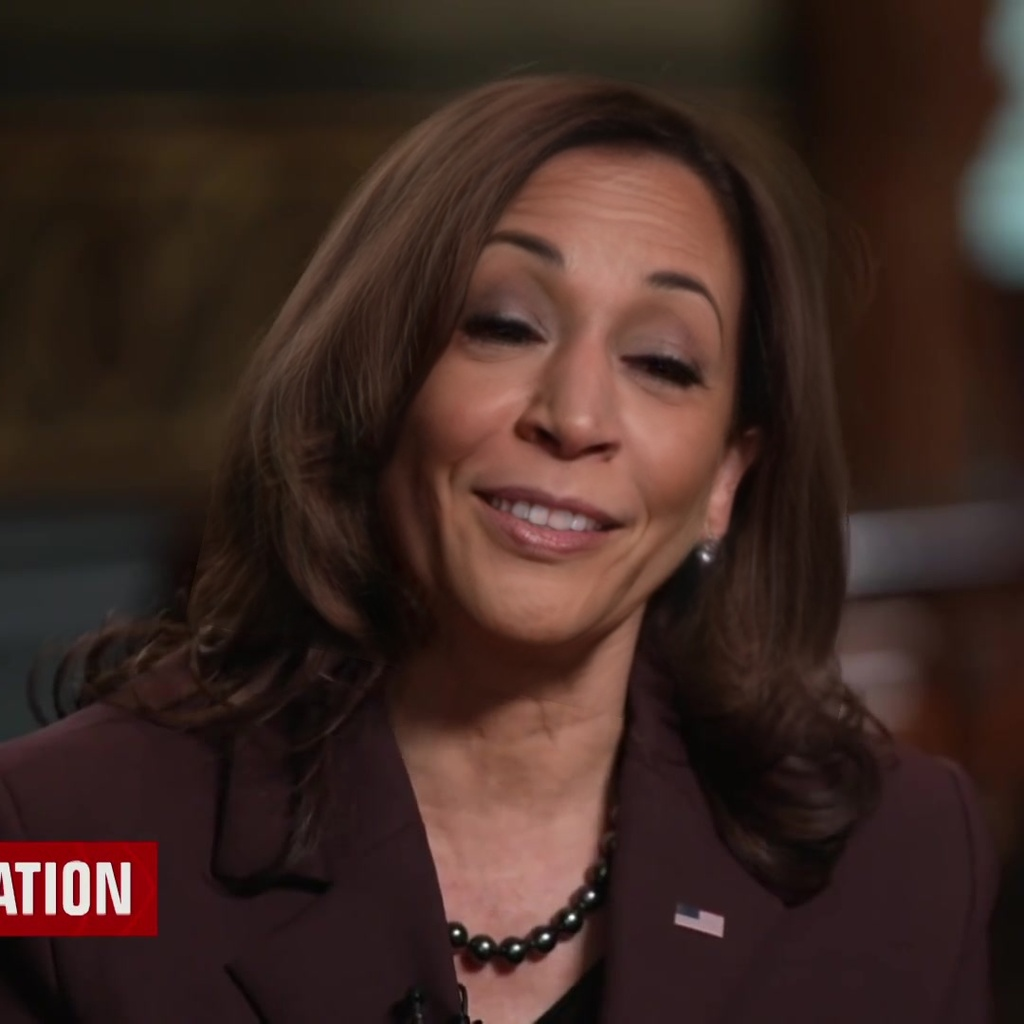
\includegraphics[width=0.095\textwidth]{resources/images/harris/smile/edit_0077.jpeg} &
%         % 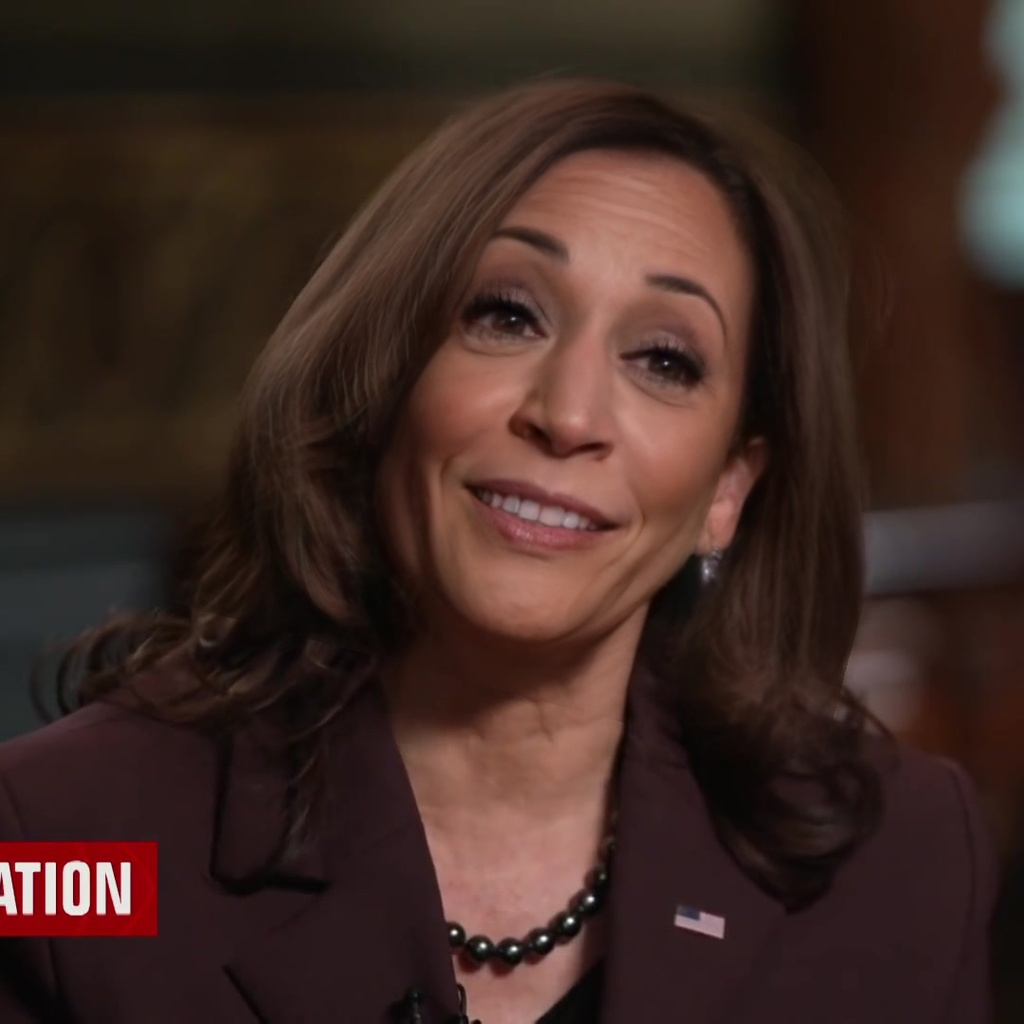
\includegraphics[width=0.095\textwidth]{resources/images/harris/smile/edit_0082.jpeg} &
%         % 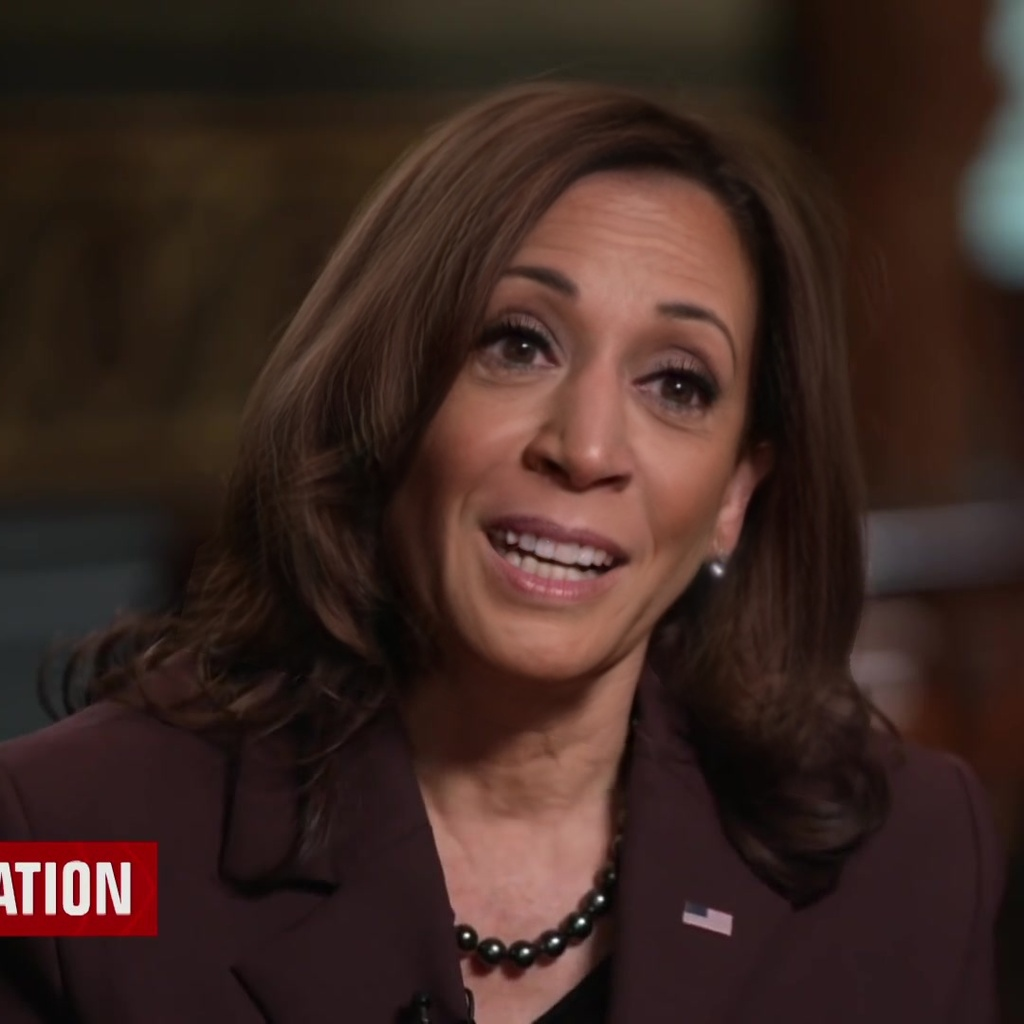
\includegraphics[width=0.095\textwidth]{resources/images/harris/smile/edit_0103.jpeg} &
%         % 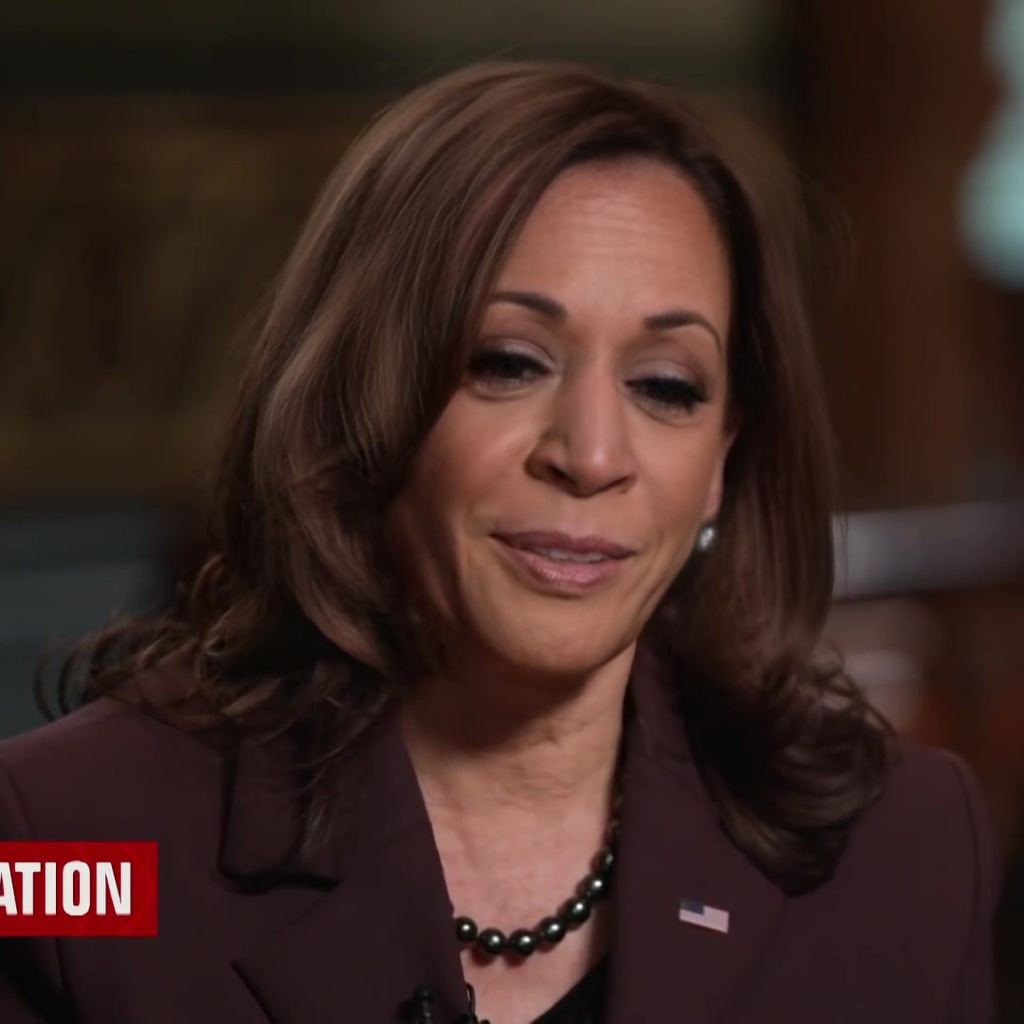
\includegraphics[width=0.095\textwidth]{resources/images/harris/smile/edit_0122.jpeg} &
%         % 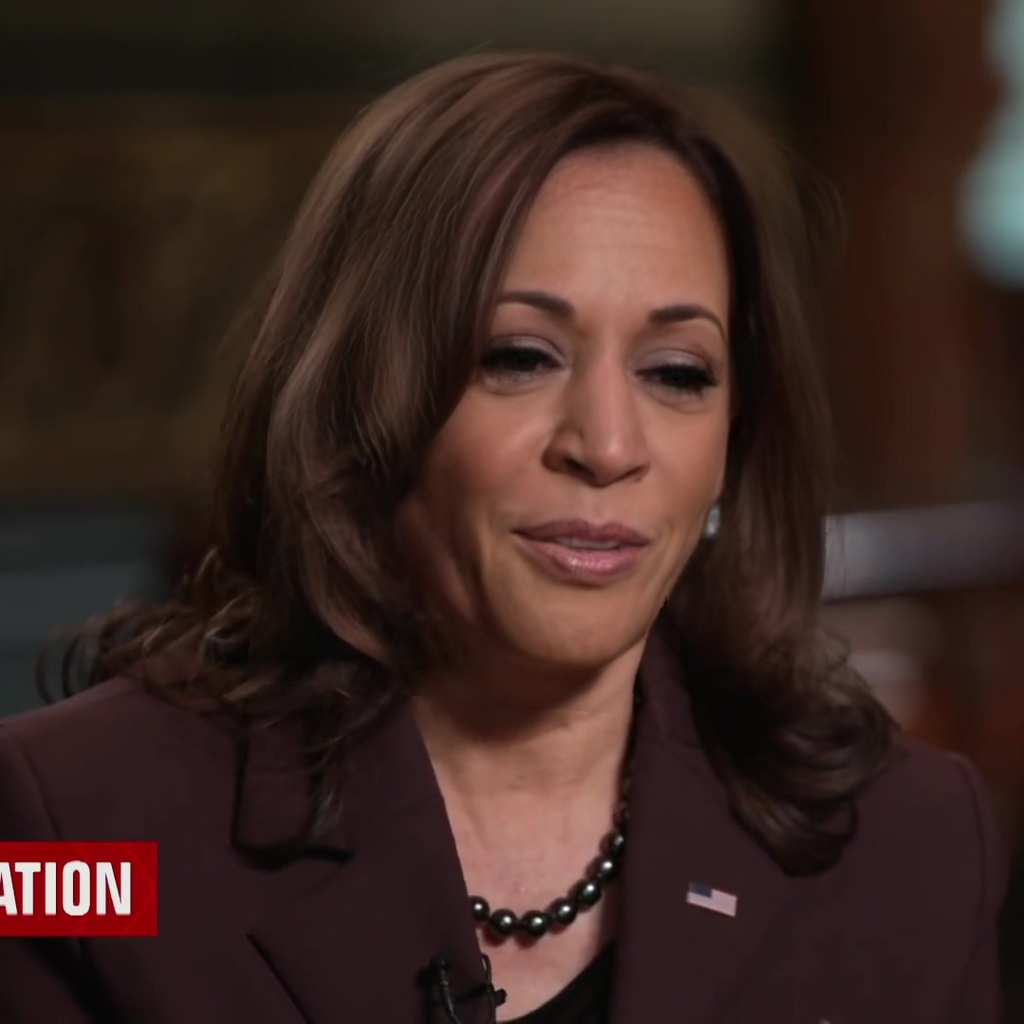
\includegraphics[width=0.095\textwidth]{resources/images/harris/smile/edit_0164.jpeg} &
%         % 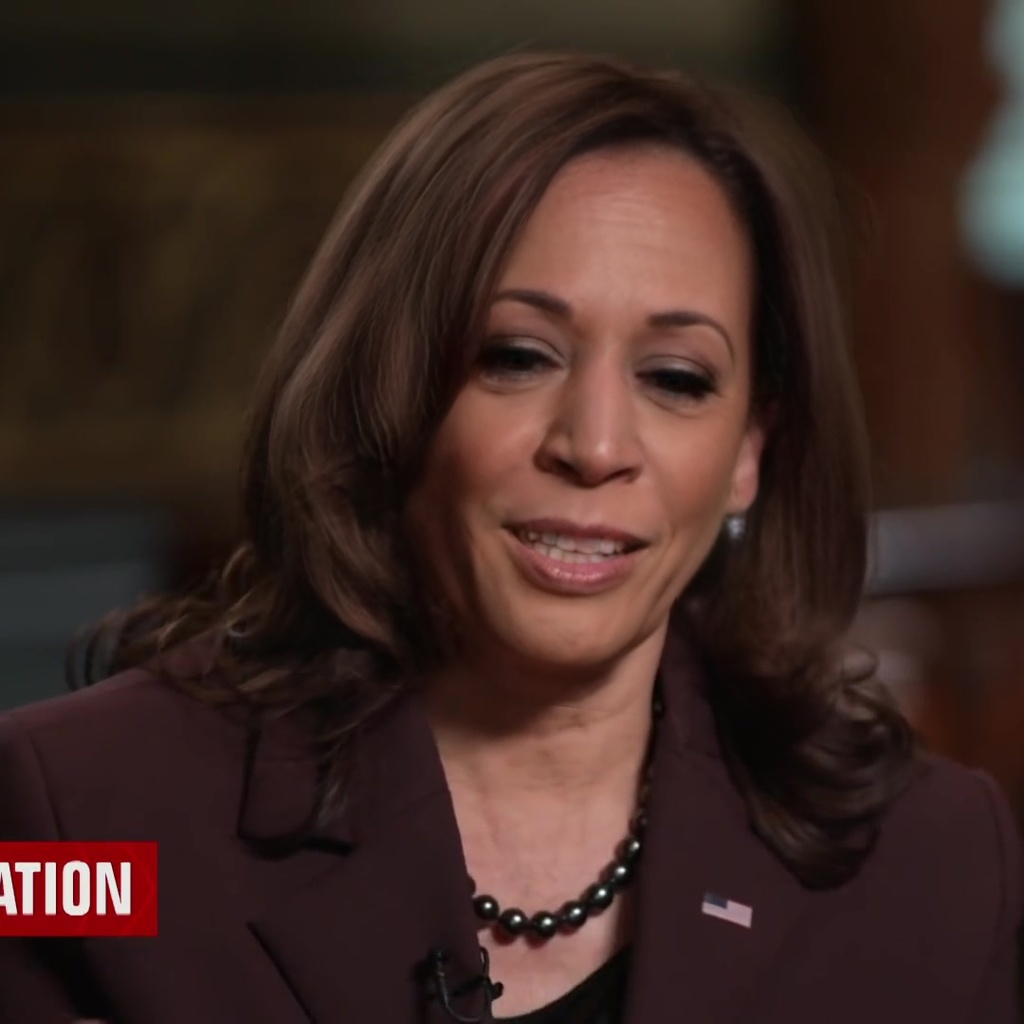
\includegraphics[width=0.095\textwidth]{resources/images/harris/smile/edit_0178.jpeg} &
%         % 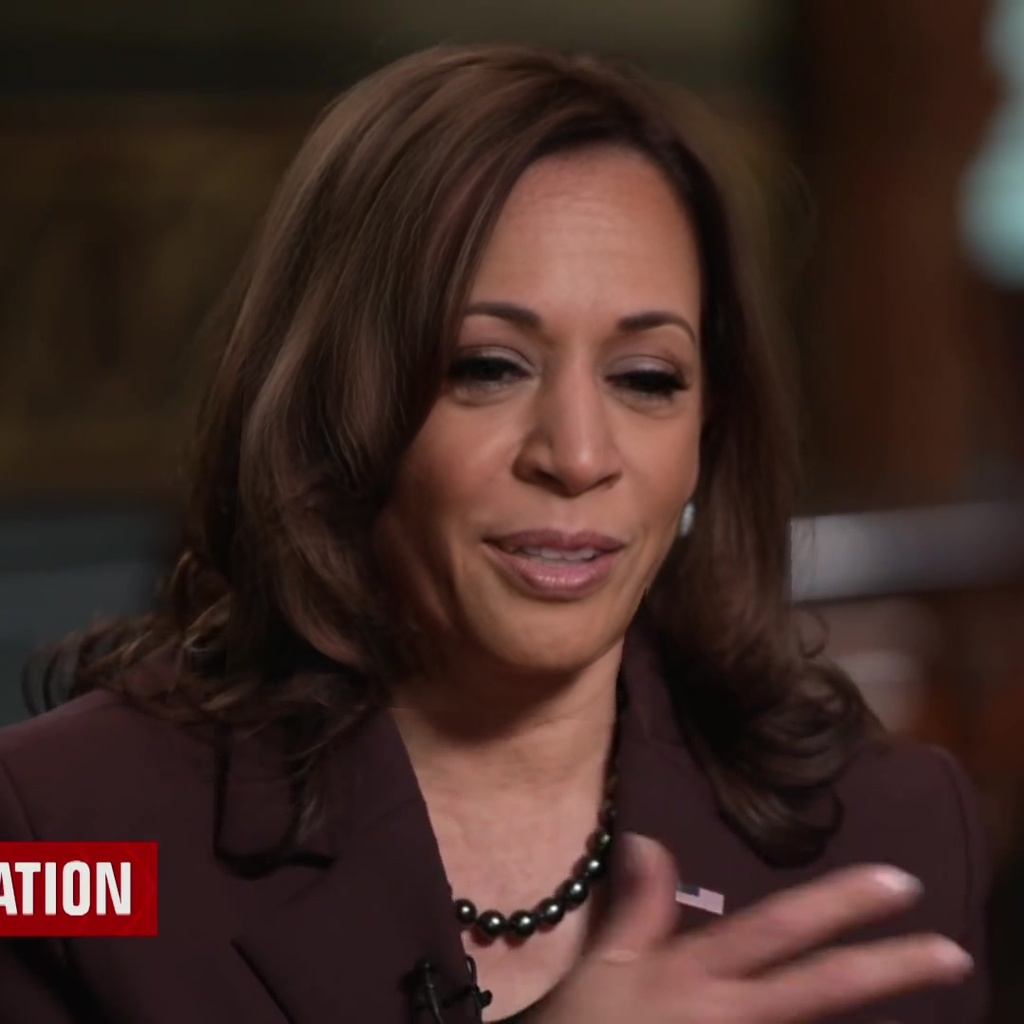
\includegraphics[width=0.095\textwidth]{resources/images/harris/smile/edit_0195.jpeg} \\
        
%         % \raisebox{0.18in}{\rotatebox{90}{$+young$}} &
%         % 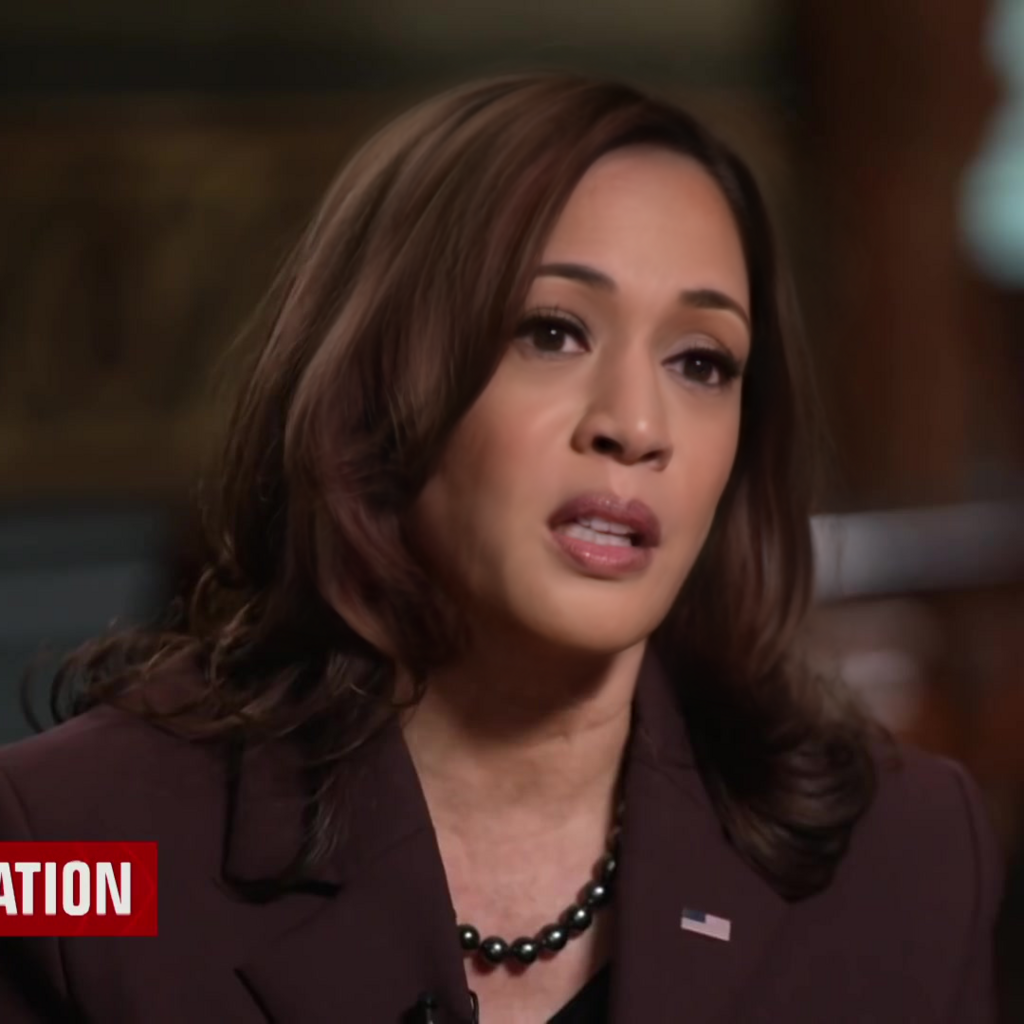
\includegraphics[width=0.095\textwidth]{resources/images/harris/young/edit_27.png} &
%         % 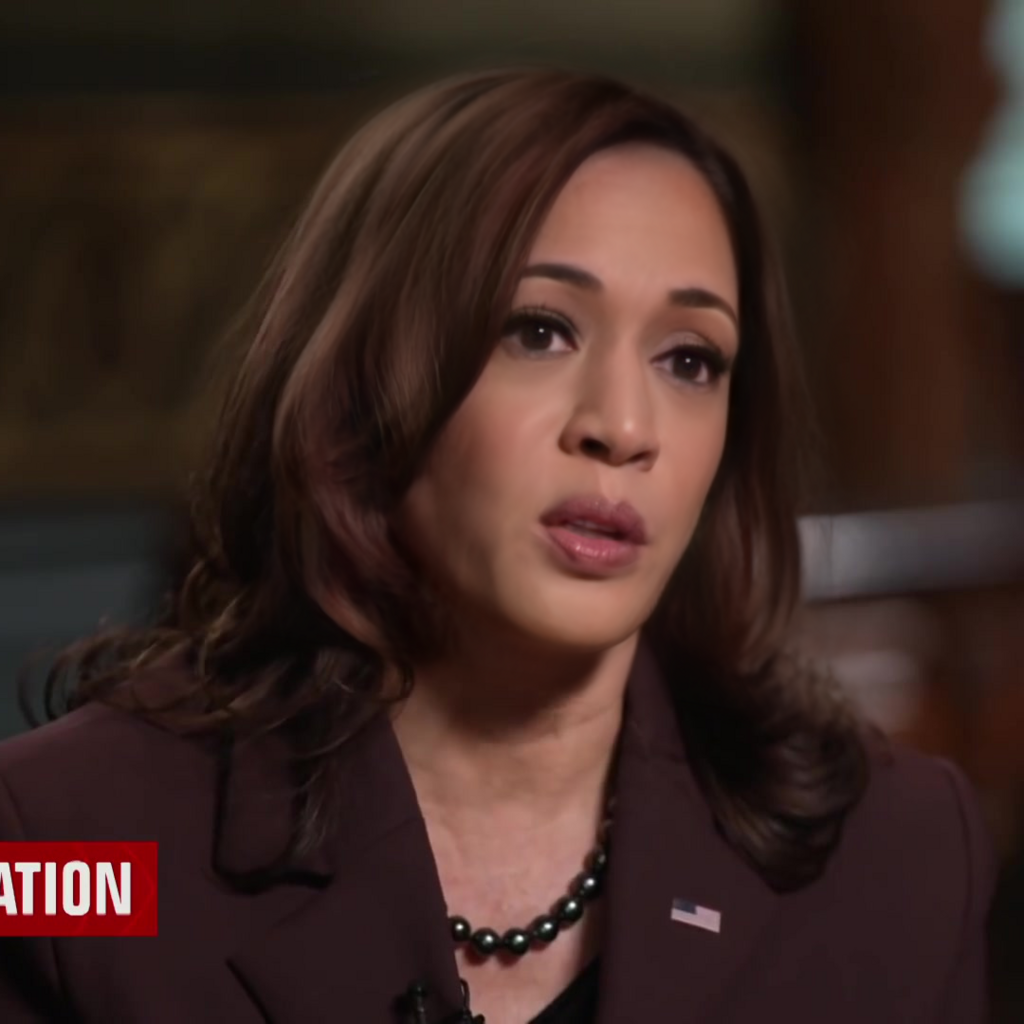
\includegraphics[width=0.095\textwidth]{resources/images/harris/young/edit_46.png} &
%         % 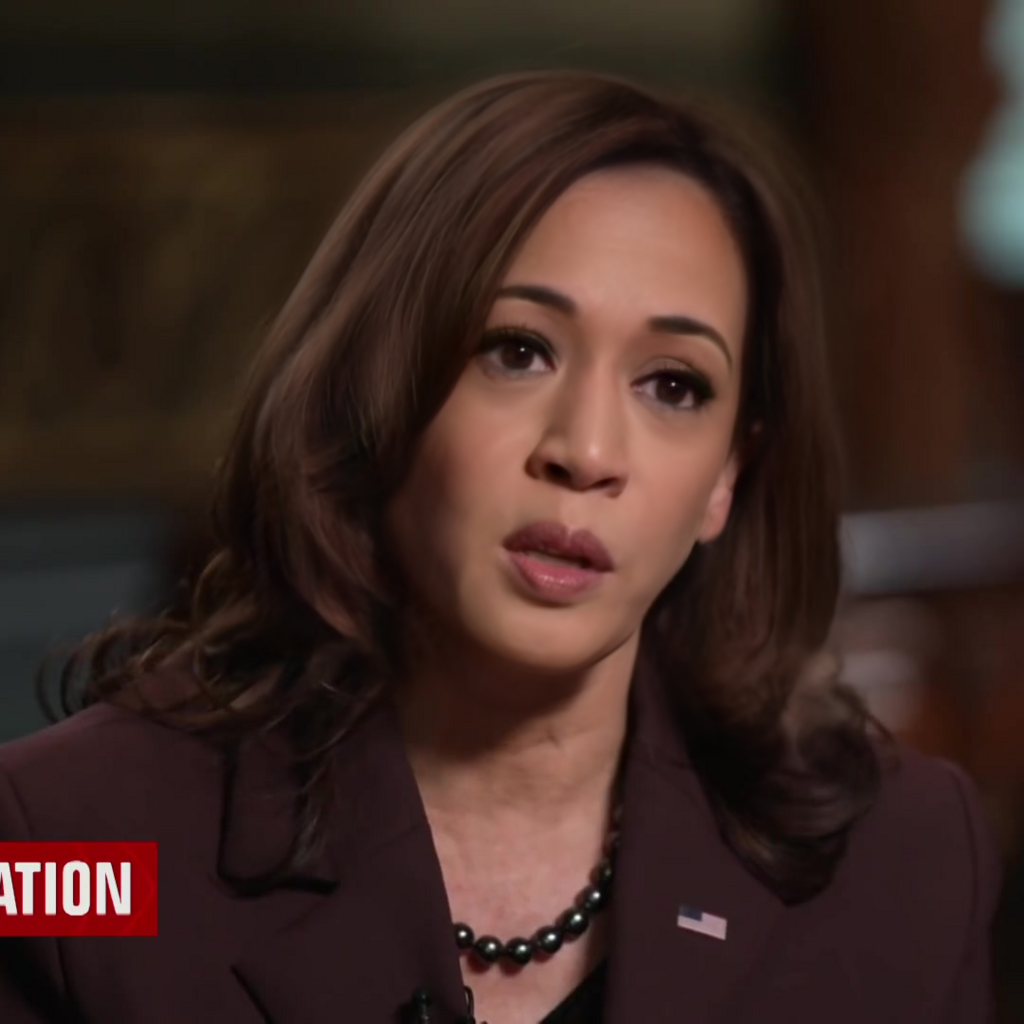
\includegraphics[width=0.095\textwidth]{resources/images/harris/young/edit_58.png} &
%         % 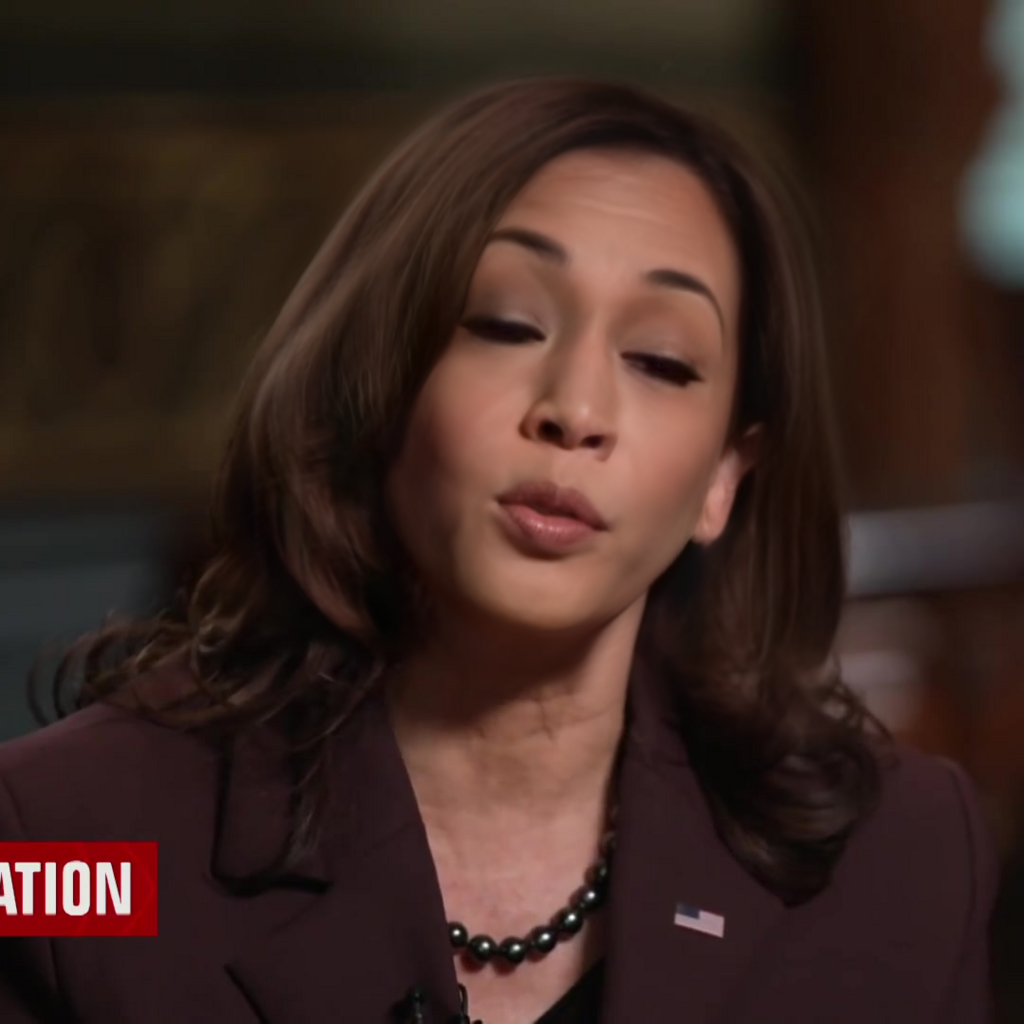
\includegraphics[width=0.095\textwidth]{resources/images/harris/young/edit_77.png} &
%         % 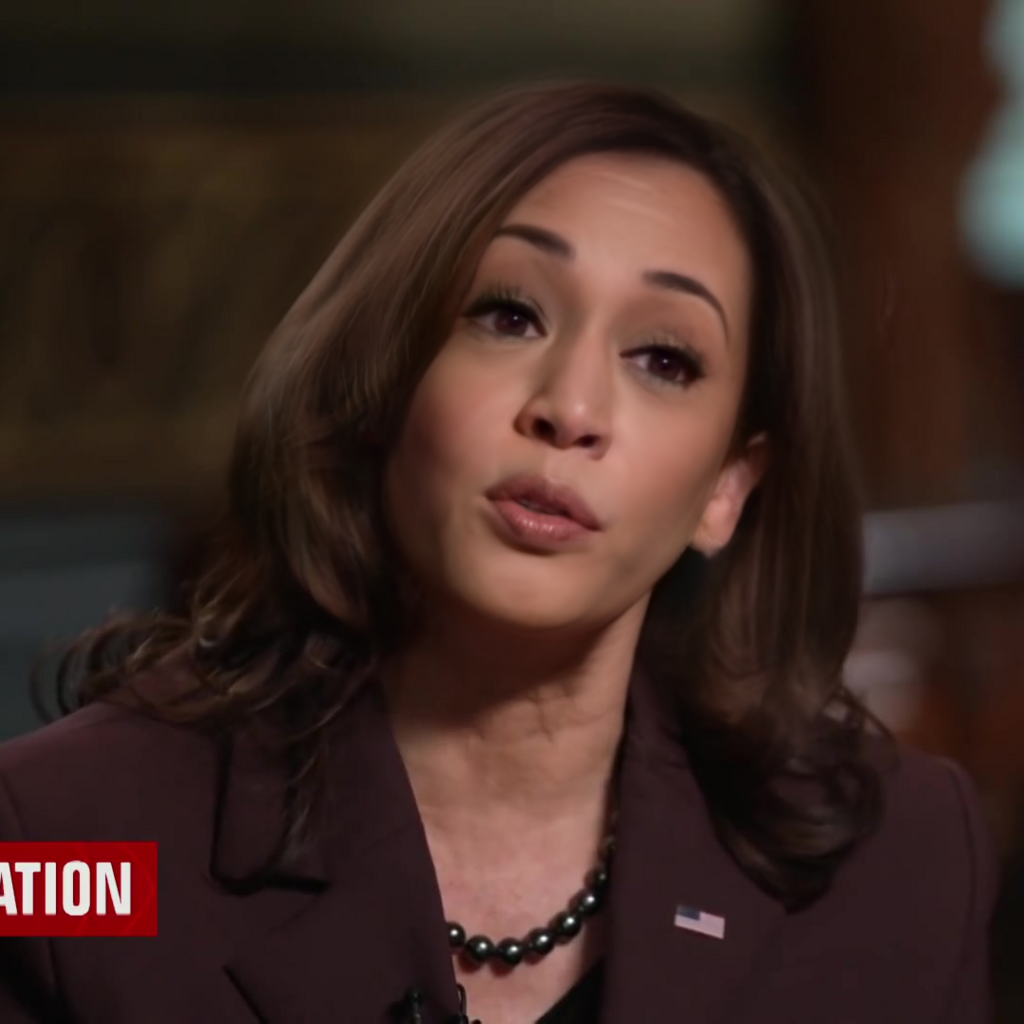
\includegraphics[width=0.095\textwidth]{resources/images/harris/young/edit_82.png} &
%         % 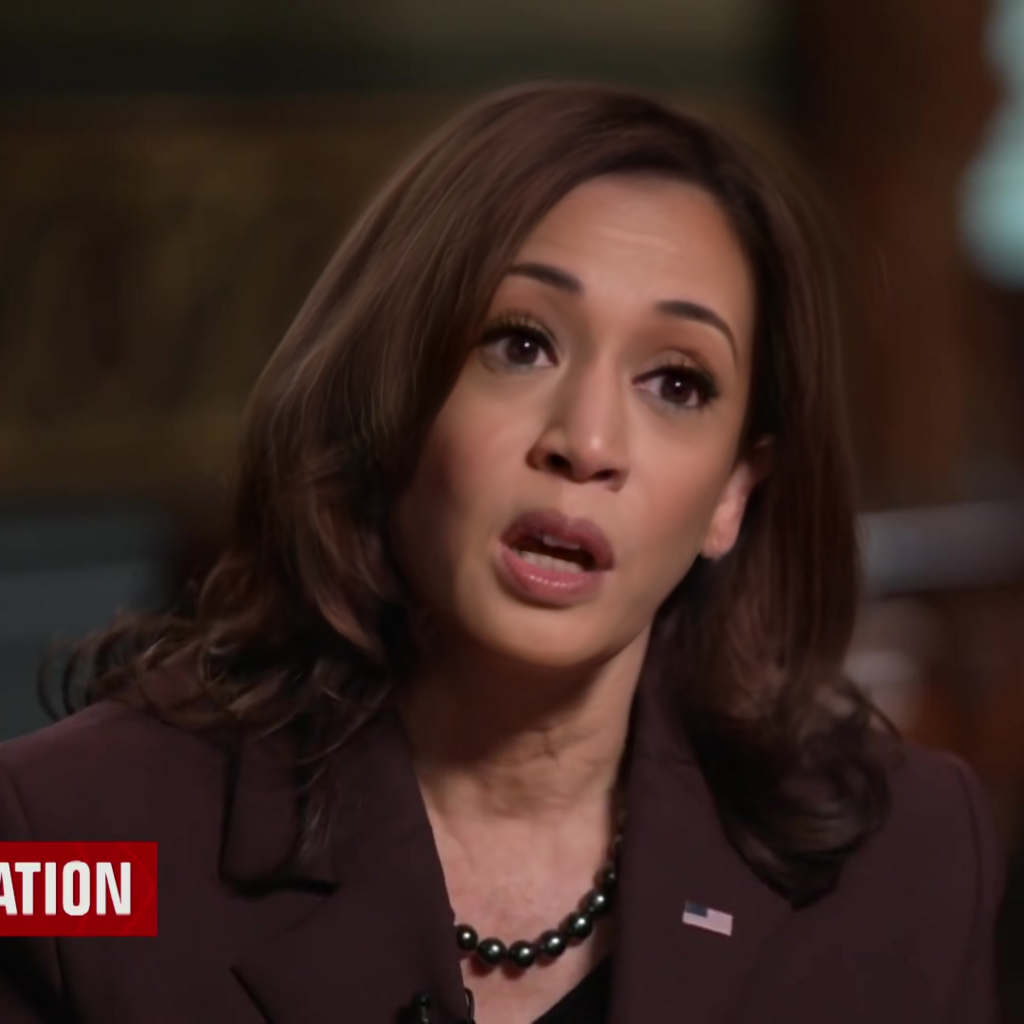
\includegraphics[width=0.095\textwidth]{resources/images/harris/young/edit_103.png} &
%         % 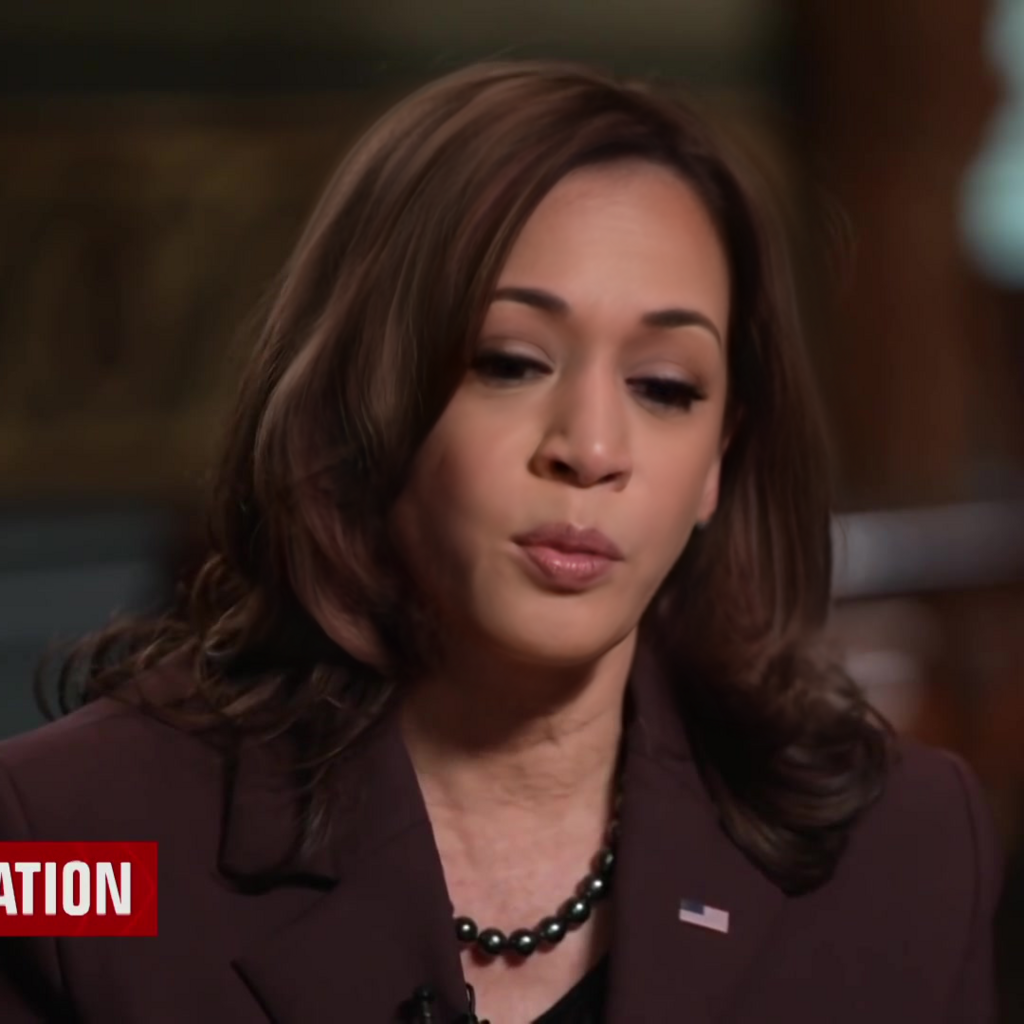
\includegraphics[width=0.095\textwidth]{resources/images/harris/young/edit_122.png} &
%         % 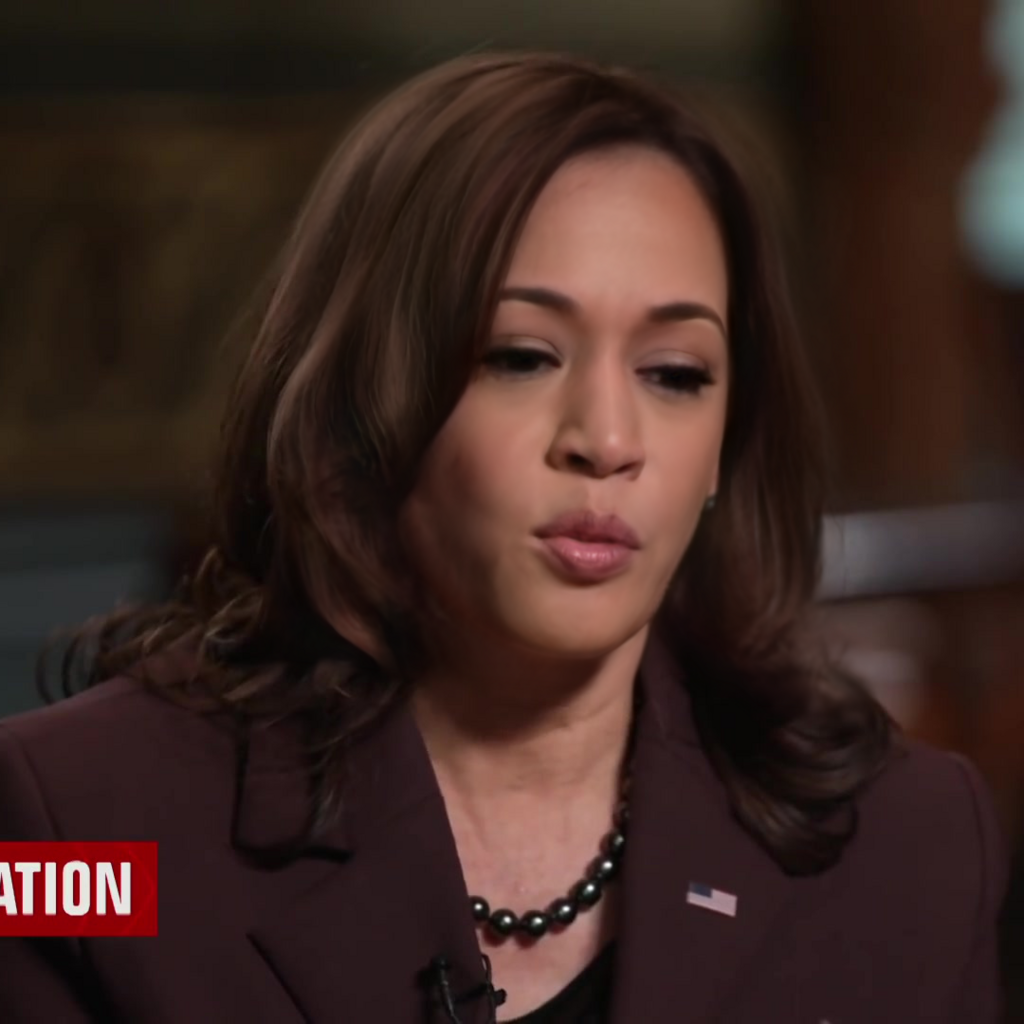
\includegraphics[width=0.095\textwidth]{resources/images/harris/young/edit_164.png} &
%         % 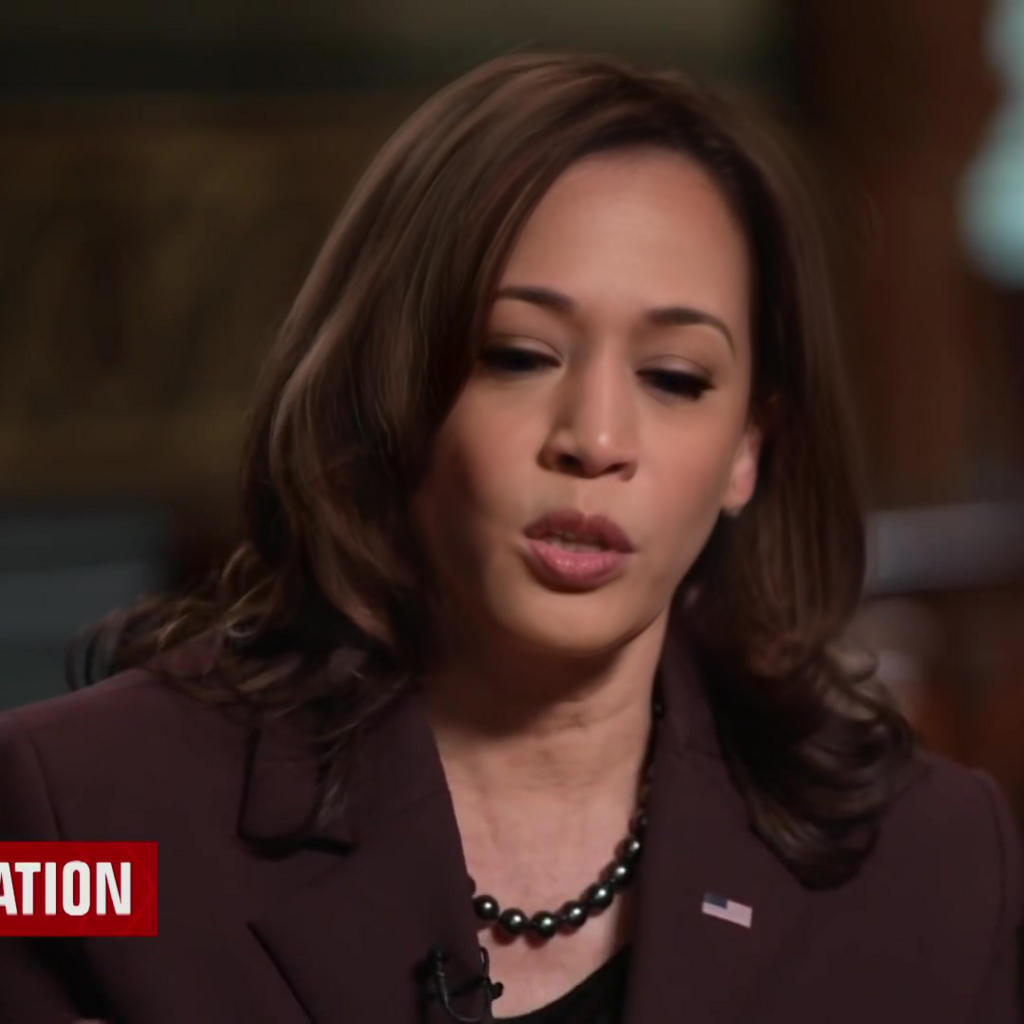
\includegraphics[width=0.095\textwidth]{resources/images/harris/young/edit_178.png} &
%         % 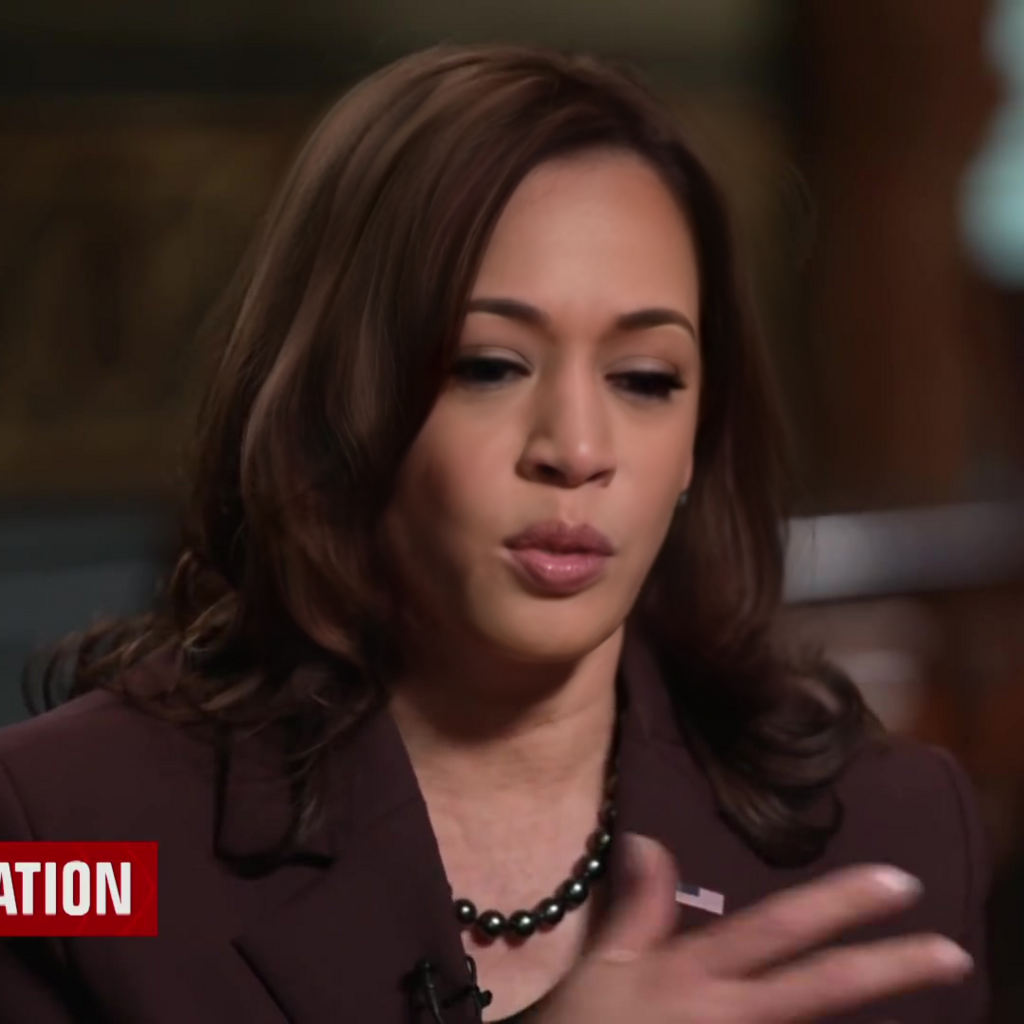
\includegraphics[width=0.095\textwidth]{resources/images/harris/young/edit_195.png} \\
        
%         % \hline
        
%         \raisebox{0.12in}{\rotatebox{90}{Original}} &
%         
\includegraphics[width=0.095\textwidth]{resources/images/OOD/source_0006.jpeg} &
%          
\includegraphics[width=0.095\textwidth]{resources/images/OOD/source_0035.jpeg} &
%         
\includegraphics[width=0.095\textwidth]{resources/images/OOD/source_0044.jpeg} &
%         
\includegraphics[width=0.095\textwidth]{resources/images/OOD/source_0054.jpeg} &                
\includegraphics[width=0.095\textwidth]{resources/images/OOD/source_0071.jpeg} &
%         
\includegraphics[width=0.095\textwidth]{resources/images/OOD/source_0074.jpeg} &
%         
\includegraphics[width=0.095\textwidth]{resources/images/OOD/source_0084.jpeg} &
%         
\includegraphics[width=0.095\textwidth]{resources/images/OOD/source_0089.jpeg} &
%         
\includegraphics[width=0.095\textwidth]{resources/images/OOD/source_0113.jpeg} &
%         
\includegraphics[width=0.095\textwidth]{resources/images/OOD/source_0138.jpeg} \\
        
%         \raisebox{0.18in}{\rotatebox{90}{$+Smile$}} &
%         
\includegraphics[width=0.095\textwidth]{resources/images/OOD/edit_0006.jpeg} &
%         
\includegraphics[width=0.095\textwidth]{resources/images/OOD/edit_0035.jpeg} &
%         
\includegraphics[width=0.095\textwidth]{resources/images/OOD/edit_0044.jpeg} &
%         
\includegraphics[width=0.095\textwidth]{resources/images/OOD/edit_0054.jpeg} &
%         
\includegraphics[width=0.095\textwidth]{resources/images/OOD/edit_0071.jpeg} &
%         
\includegraphics[width=0.095\textwidth]{resources/images/OOD/edit_0074.jpeg} &
%         
\includegraphics[width=0.095\textwidth]{resources/images/OOD/edit_0084.jpeg} &
%         
\includegraphics[width=0.095\textwidth]{resources/images/OOD/edit_0089.jpeg} &
%         
\includegraphics[width=0.095\textwidth]{resources/images/OOD/edit_0113.jpeg} &
%         
\includegraphics[width=0.095\textwidth]{resources/images/OOD/edit_0138.jpeg} \\

%         % \\

%         %& Frame 1 & Frame 2 & Frame 3 & Frame 4 & Frame 1 & Frame 2 & Frame 3 & Frame 4
        
%     \end{tabular}
    
%     }
%     \vspace{-0.225cm}
%     \caption{Video editing using our proposed pipeline. Our framework can successfully apply consistent semantic manipulations to challenging talking-head videos, without requiring any temporal components or losses.}
%     %\vspace{-0.225cm}
%     \label{fig:ood}
% \end{figure*}


\begin{figure}
    \centering
    \setlength{\belowcaptionskip}{-6pt}
    \setlength{\tabcolsep}{0.5pt}
    {
    \begin{tabular}{ccccc}
        
        \vspace{-0.0615cm}
        
        \raisebox{0.15in}{\rotatebox{90}{Original}} &
        \includegraphics[width=0.11\textwidth]{resources/images/OOD/source_0006.jpeg} &
         \includegraphics[width=0.11\textwidth]{resources/images/OOD/source_0035.jpeg} &
        \includegraphics[width=0.11\textwidth]{resources/images/OOD/source_0054.jpeg} &                \includegraphics[width=0.11\textwidth]{resources/images/OOD/source_0071.jpeg} \\
        
        \raisebox{0.18in}{\rotatebox{90}{$+Smile$}} &
        \includegraphics[width=0.11\textwidth]{resources/images/OOD/edit_0006.jpeg} &
        \includegraphics[width=0.11\textwidth]{resources/images/OOD/edit_0035.jpeg} &
        \includegraphics[width=0.11\textwidth]{resources/images/OOD/edit_0054.jpeg} &
        \includegraphics[width=0.11\textwidth]{resources/images/OOD/edit_0071.jpeg} \\ \\
        
        \raisebox{0.15in}{\rotatebox{90}{Original}} &
        \includegraphics[width=0.11\textwidth]{resources/images/OOD/source_0074.jpeg} &
        \includegraphics[width=0.11\textwidth]{resources/images/OOD/source_0084.jpeg} &
        \includegraphics[width=0.11\textwidth]{resources/images/OOD/source_0113.jpeg} &
        \includegraphics[width=0.11\textwidth]{resources/images/OOD/source_0138.jpeg} \\
        
        \raisebox{0.18in}{\rotatebox{90}{$+Smile$}} &
        \includegraphics[width=0.11\textwidth]{resources/images/OOD/edit_0074.jpeg} &
        \includegraphics[width=0.11\textwidth]{resources/images/OOD/edit_0084.jpeg} &
        \includegraphics[width=0.11\textwidth]{resources/images/OOD/edit_0113.jpeg} &
        \includegraphics[width=0.11\textwidth]{resources/images/OOD/edit_0138.jpeg} \\

        % \\

        %& Frame 1 & Frame 2 & Frame 3 & Frame 4 & Frame 1 & Frame 2 & Frame 3 & Frame 4
        
    \end{tabular}
    
    }
    \vspace{-0.225cm}
    \caption{Out-of-domain video editing. Our method can seamlessly adapt to other facial domains, and can handle challenging poses and expressions.}
    %\vspace{-0.225cm}
    \label{fig:ood}
\end{figure}
In \cref{fig:ood} we showcase our ability to edit out-of-domain videos. Both the encoder and PTI can seamlessly adapt to animated faces. Furthermore, the alignment of fine-tuned StyleGAN models ensures we can re-use the same editing directions, as previously demonstrated by \cite{gal2021stylegannada}, \cite{alaluf2021hyperstyle} and \cite{zhu2021mind}.


\subsection{Quantitative Results}
\label{sec:quantitative}

We next evaluate our method quantitatively. As previously outlined, we expect that encoder-based methods will be smoother at the local level, avoiding the jitter induced by optimization techniques. On the other hand, we expect them to display considerable identity drift at the global scale - with the minor inversion inconsistencies between the frames building up over time. To validate our intuition and evaluate the temporal coherence of videos, we propose two novel metrics: temporally-local (TL-ID) and temporally-global (TG-ID) identity preservation. 


In the first case, TL-ID, we aim to evaluate the video's consistency at the local level. We do so by employing an off-the-shelf identity detection network~\cite{deng2019arcface} to evaluate the identity similarity between pairs of adjacent video frames. To account for the effect of inconsistencies in the identity network itself, we normalize these identity preservation scores by the similarity score of each pair of frames in the original video. Finally, we average the normalized scores over the entire video, and then once again over a set of videos.
Higher TL-ID scores indicate that the method produces \textit{smooth} results, without considerable \textit{local} identity jitter. 


Our second metric, TG-ID, employs the same identity detection network and averaging scheme to evaluate the similarity between all possible pairs of video frames, not necessarily adjacent. This metric aims to capture longer-range coherence and identify slow, but consistent identity drift.
For both metrics, a score of $1$ would indicate that the method successfully maintains the identity consistency of the original video.
Note that both metrics only compare frames \textit{within} a given video. As such, they do not measure the similarity of the inversions to those of the original video. Rather, we focus on quantifying the temporal consistency of these inversions and the editing operations they support.

We utilize both metrics to evaluate our method against the baseline PTI~\cite{roich2021pivotal}, as well as Latent Transformer~\cite{yao2021latent} which makes use of a pre-trained pSp~\cite{richardson2020encoding} encoder for inversion. The results are shown in \cref{tb:temporal_id}. As expected, encoder-based methods outperform the optimization-based method on local consistency, demonstrating that they do indeed provide a smooth prior. Moreover, combining an encoder with PTI results in local consistency which is just shy of $1$, showing that the proposed pipeline is sufficient to inherit almost all temporal consistency from the source video.


On the global front, PTI improves identity preservation over longer time spans. While editing is still susceptible to the inconsistencies of the local pivots, the encoder-based methods lead to an identity drift that eventually surpasses the local jitter. PTI, meanwhile, constantly re-aligns the identity to that of the source video, avoiding longer term drift. Notably, PTI does demonstrate some drop in global performance when compared to the local score. We hypothesize that this originates in the increased distance between pivots when optimizing around distant frames.
By leveraging PTI, our method can similarly maintain a high level of global consistency, and even outperform PTI thanks to more consistent pivot codes.

\begin{table}[]
    \centering
\begin{tabular}{c | c | c }
        \toprule
        Model & TL-ID $\uparrow$ & TG-ID $\uparrow$ \\
        \midrule
        Latent Transformer & 0.976 & 0.811 \\
        PTI (optimization) & 0.933 & 0.901 \\
        Ours & \textbf{0.996} & \textbf{0.933} \\
        \bottomrule
\end{tabular}

    \caption{Temporal consistency metrics. Encoder based methods display improved identity preservation at the local (adjacent frame) level, but show considerable identity drift over time. PTI, preserves a greater degree of global identity, at the cost of local jitter from inconsistent pivots. Our pipeline outperforms the alternatives and achieves a local-identity preservation score which is nearly equal to the original video (1), demonstrating our ability to maintain a high degree of consistency.}
    \vspace{-0.35cm}
    \label{tb:temporal_id}
    
\end{table}

\subsection{Ablation Study}
\label{sec:ablation}

We further demonstrate the benefits of each component in our pipeline by conducting an ablation study. In \cref{fig:ablation} we show key frames from a video edited using our method when crucial steps of the pipeline are removed or replaced. We showcase the effects of replacing the encoder with an optimization method (w/o e4e), removing the PTI generator-tuning step, replacing the stitching-tuning step by {\naive}ly pasting the edited image inside the segmentation mask, and finally our full pipeline.

Without an encoder, the edited frames become inconsistent when the face undergoes considerable movement or changes in expression. Without PTI, frames are less faithful to the original video, stitching performance suffers, and identity changes over longer time periods.
Without stitching, artifacts appear around the hair and borders of the segmentation mask (\ie the edge of the face). Our full method maintains both local and long term consistency, and seamlessly melds the edited region into the original frame.

\begin{figure}
\setlength{\tabcolsep}{0.5pt}
    \centering
    { \small 
\begin{tabular}{ccccc}
Original & w/o e4e & w/o PTI & w/o Stitching & Ours \\
\raisebox{-.32\totalheight}{\includegraphics[width=0.2\columnwidth]{resources/images/ablation_micheal/original/source_0100.jpeg}} &
\raisebox{-.32\totalheight}{\includegraphics[width=0.2\columnwidth]{resources/images/ablation_micheal/no_e4e/optimized_0100.jpeg}} &
\raisebox{-.32\totalheight}{\includegraphics[width=0.2\columnwidth]{resources/images/ablation_micheal/no_pti/optimized_0100.jpeg}} &
\raisebox{-.32\totalheight}{\includegraphics[width=0.2\columnwidth]{resources/images/ablation_micheal/no_stitching/edit_0100.jpeg}} &
\raisebox{-.32\totalheight}{\includegraphics[width=0.2\columnwidth]{resources/images/ablation_micheal/ours/optimized_0100.jpeg}} \\

\raisebox{-.32\totalheight}{\includegraphics[width=0.2\columnwidth]{resources/images/ablation_micheal/original/source_0083.jpeg}} &
\raisebox{-.32\totalheight}{\includegraphics[width=0.2\columnwidth]{resources/images/ablation_micheal/no_e4e/optimized_0083.jpeg}} &
\raisebox{-.32\totalheight}{\includegraphics[width=0.2\columnwidth]{resources/images/ablation_micheal/no_pti/optimized_0083.jpeg}} &
\raisebox{-.32\totalheight}{\includegraphics[width=0.2\columnwidth]{resources/images/ablation_micheal/no_stitching/edit_0083.jpeg}} &
\raisebox{-.32\totalheight}{\includegraphics[width=0.2\columnwidth]{resources/images/ablation_micheal/ours/optimized_0083.jpeg}} \\

\raisebox{-.32\totalheight}{\includegraphics[width=0.2\columnwidth]{resources/images/ablation_micheal/original/source_0030.jpeg}} &
\raisebox{-.32\totalheight}{\includegraphics[width=0.2\columnwidth]{resources/images/ablation_micheal/no_e4e/optimized_0030.jpeg}} &
\raisebox{-.32\totalheight}{\includegraphics[width=0.2\columnwidth]{resources/images/ablation_micheal/no_pti/optimized_0030.jpeg}} &
\raisebox{-.32\totalheight}{\includegraphics[width=0.2\columnwidth]{resources/images/ablation_micheal/no_stitching/edit_0030.jpeg}} &
\raisebox{-.32\totalheight}{\includegraphics[width=0.2\columnwidth]{resources/images/ablation_micheal/ours/optimized_0030.jpeg}} \\

\raisebox{-.32\totalheight}{\includegraphics[width=0.2\columnwidth]{resources/images/ablation_micheal/original/source_0000.jpeg}} &
\raisebox{-.32\totalheight}{\includegraphics[width=0.2\columnwidth]{resources/images/ablation_micheal/no_e4e/optimized_0000.jpeg}} &
\raisebox{-.32\totalheight}{\includegraphics[width=0.2\columnwidth]{resources/images/ablation_micheal/no_pti/optimized_0000.jpeg}} &
\raisebox{-.32\totalheight}{\includegraphics[width=0.2\columnwidth]{resources/images/ablation_micheal/no_stitching/edit_0000.jpeg}} &
\raisebox{-.32\totalheight}{\includegraphics[width=0.2\columnwidth]{resources/images/ablation_micheal/ours/optimized_0000.jpeg}} \\

\end{tabular}
}


\caption{Qualitative demonstration of the importance of our pipeline components. Replacing the encoder with an optimization step results in poor editing consistency. Without PTI, identity drifts over time, and stitching performance deteriorates. Replacing stitching with a mask-based blending scheme results in visual artifacts, such as sharp transitions in hair regions. Our full pipeline successfully avoids these pitfalls and generates a consistent video.}
\label{fig:ablation}
\end{figure}